\documentclass{article}
\usepackage{bookman}
\renewcommand{\familydefault}{\sfdefault}
\usepackage{pdfpages}
\usepackage{fancyhdr}
\usepackage{graphicx}
\usepackage{url}
\usepackage{enumitem}
\usepackage[a4paper]{geometry}
%\geometry{showframe}
%\geometry{left=2.5cm}
\usepackage[utf8]{inputenc}% Brug af æ, ø og å
\usepackage{etoolbox}

\usepackage{adjustbox}
\usepackage{longtable}
\usepackage{verbatim}
\usepackage{pdflscape}
\usepackage{tocloft}

\usepackage{fancybox}
\usepackage[T1]{fontenc}
\usepackage{ragged2e}

%fancy style for pagenumbers
\fancypagestyle{customplain}{%
\fancyhf{}%
\fancyhf[cf]{\thepage}%
\setlength{\footskip}{80pt}
\renewcommand*\headrulewidth{0pt}}

\fancypagestyle{appendixplain}{%
\fancyhf{}%
\fancyhf[cf]{\thepage}%
\setlength{\footskip}{90pt}
\renewcommand*\headrulewidth{0pt}}

\newenvironment{newab}
		{\small
			\begin{center}
				\bfseries \abstractname\vspace{-.5em}\vspace{0pt}
			\end{center}
			\list{}{
				\setlength{\leftmargin}{.5cm}%
				\setlength{\rightmargin}{\leftmargin}%
			}%
			\item\relax}
		%{\endlist}
		
\newenvironment{dummy}{}

\AtBeginDocument{                                               
  \renewcommand{\cftsecleader}{\cftdotfill{\cftsecdotsep}}    
  \renewcommand\cftsecdotsep{\cftdot}                         
  \renewcommand\cftsubsecdotsep{\cftdot}                      
  \renewcommand{\cftfigleader}{\cftdotfill{\cftsecdotsep}}
  \renewcommand{\cfttableader}{\cftdotfill{\cftsecdotsep}}
}

\begin{document}
\setcounter{page}{1}

\includepdf[fitpaper,pages=-,pagecommand={\thispagestyle{empty}}]{posterv2.pdf}
\cleardoublepage

\newpage\null\thispagestyle{empty}\newpage
\cleardoublepage

\newgeometry{left=2.5cm}
\thispagestyle{empty}
% !TEX root = ../rapport.tex

% Dette er LaTeX-versionen af titelbladet for tek-nat-basis-rapporter 2004 efterår
% Filen kræver:
% Universitetets logo:  aau-logo.png (for LaTeX) eller aau-logo.ps (for LaTeX)
% Synopsis: En fil ved navn synopsis.tex

% Udarbejdet af: Hans Hüttel (hans@cs.auc.dk) 21. maj 2003
% Rettet af Morten Christophersen (mortench@tnb.aau.dk) 30. nov 2004 (ændret til nyt design 2004 efterår)

\begin{nopagebreak}
{\samepage

\begin{tabular}{r}
	\parbox{\textwidth}
	{  
		\raisebox{-9mm}{
\includegraphics[height=3cm]{formalities/aau_uk_studentreport_blue.png}}
		\hspace{3.7cm} \parbox{0cm}
		{
			\begin{tabular}{l}
			{\small \textbf{Aalborg University,}}\\
			{\small \textbf{Department of Computer Science}}\\
			
			{\small Selma Lagerlöfsvej 300} \\
			{\small Phone 99 40 72 28} \\
			{\small \url{http://www.cs.aau.dk}}
			\end{tabular}
		}
		\vspace{0cm}
	}
\end{tabular}

\begin{tabular}{cc}
\parbox{8cm}{

\begin{description}

\item {\textbf{Title of Literature Review:}}\\
Toward Cross-device Natural User Interactions with Large
\item {\textbf{Title of Research Paper:}}\\ 
Comparison of Push Techniques for Cross-Device Interaction Between Mobile Devices and Large Displays

\end{description}

\parbox{8cm}{

\begin{description}[itemsep=10pt, topsep=12pt, partopsep=0pt]
\item {\textbf{Project period:}}\\
   IS9, Autumn Semester 2015\\
   1st September 2015 \\
   to 18th February 2016
  \hspace{4cm}
\item {\textbf{Group:}}\\
  IS903E15
  \hspace{4cm}
\item {\textbf{Participants:}} \\
  Bjarke M. Lauridsen\\
  Ivan S. Penchev\\
  Elias Ringhauge\\
  Eric V. Ruder
  \hspace{2cm}
\item {\textbf{Supervisor:}}\\
  Jeni Paay
\end{description}
}
\begin{description}
\item { Circulation: 2 }
\item { Number of pages: 49 }
\item { Appendices: 8 + 1 CD} 
\end{description}
\vfill } &
\parbox{7cm}{
  \vspace{.15cm}
  \hfill 
  \begin{tabular}{l}
  {\textbf{Abstract:}}\bigskip \\
  \fbox{
    \parbox{6.5cm}{\bigskip
     {\vfill{\small % !TEX root = ../rapport.tex

This report documents the development of a smartphone application that utilizes virtual reality to replicate a physical game experience.
For this project it was decided to use Jenga as a case study.

The project evaluates several smartphone components in order to determine which are usable for virtual reality.
Of the sensor components evaluated it was found that the gyroscope, accelerometer and compass were suitable, while the suitable feedback components were found to be the display, speakers and vibrator.

The application was developed to obtain a virtual reality representation of the Jenga game experience.
It allows the player to rotate the in-game camera in three dimensions in the virtual environment.
     \bigskip}}
     }}
   \end{tabular}}
\end{tabular}}
\vspace{1.3cm}
\end{nopagebreak}

\restoregeometry
\cleardoublepage

\newpage\null\thispagestyle{empty}\newpage
\cleardoublepage

\newpage
\tableofcontents
\newpage
\cleardoublepage

\newpage\null\thispagestyle{empty}\newpage
\cleardoublepage

\section*{Preface}
\addcontentsline{toc}{section}{Preface}
This collection of papers is the result of our 9th semester work, as software engineers, in Human Computer Interaction, at the Department of Computer Science at Aalborg University.

The theme of our project is cross-device interaction between mobile devices and large displays. Here we present two papers. First a literature review, then a research paper. 

A CD containing the source code of the developed systems is supplied together with this report. The CD also contains a digital copy of this report as well as appendices with e.g. interview transcriptions. Additionally, it contains all logged numbers used for the quantitative analysis, enclosed as database exports.

We would like to thank Jeni Paay, Associate Professor at Aalborg University, for providing ongoing feedback and guidance throughout the project
\cleardoublepage

\newpage\null\thispagestyle{empty}\newpage
\cleardoublepage

% !TEX root = ../paper.tex
\section{Introduction} \label{sec:introduction}
The evolution of ways people interact with the digital is noteworthy considering the short life-span of computing. How we use our devices, which devices we use, and the context in which we use them has been continually under transformation. From portable personal computers, originally considered mostly for specialized field applications, such accountancy, military use, or for sales representatives, which addressed mobility of a person's workspace, to modern hand-held devices which presented, their users, such degree of freedom that ultimately workspaces are starting to fade. This expansion has not only increased mobile computing due to greater convenience, but also made it widespread.\cite{Francis:1997} \\

As numerous divergent devices are being adopted in different domains and context, cross-device interaction is currently becoming more important and relevant, as people take their hand-held devices into situations where other technologies are active. This ubiquitous presence of devices means that it can be leverage to enhance everyday situations in all kind of places. Imagine if a public display can morph from one-way broadcast device that merely show visual content to a two-way interaction device that provides more engaging and immersive experience. Given this emergence of cross-device communication opportunities prompts a need to understand how different interaction techniques perform in use, e.g. in terms of how easily, quickly and accurately, or in terms of how enjoyable or satisfying it's it to interact in this way. \\

Research in the area of cross-device interaction has been trying to keep up with the changing trends, earliest examples are in the late 90's, within ubiquitous computing, with Rekimoto's work,  he argued for, what he called, multi computed user interface and that interaction technique must overcome the boundaries among devices in multi-device settings\cite{Rekimoto:1998}.

Recent HCI research has focused on how to include in cross-device interaction an more natural modality contributing to what should be know as cross-device natural user interaction.  Some researchers used spatial information \cite{Marquardt:2011, Marquardt:2012}, others used touch \cite{Seifert:2012}, or combined touch with air gestures \cite{Bragdon:2011} . But we still have limited understanding of how to design cross-device natural user interaction techniques and also we are missing on quantitative studies of the aforementioned.\\

Inspired by the opportunities presented of such challenges, this paper reports on a quantitative study between four different cross-device natural user interaction techniques for data transfer between hand-held device and large displays.

We discover that out of the four techniques we developed and implemented, \swipe was the most precise and effective technique, which could be used to create more interesting and effective natural user interfaces with. We uncover that the need for precision comes at a great cost in regards to effectiveness, and should be side-stepped\todo{contrast this with any other that was strongest at some aspect?? also, be clear about what you mean by effective.} if possible while designing and implementing the application.  


\cleardoublepage

\newpage\null\thispagestyle{empty}\newpage
\cleardoublepage

%\section*{Paper I: Literature Review}
\addcontentsline{toc}{section}{Paper 1: Literature Review}

%\newlength{\drop}
\begin{dummy}

		\drop=0.1\textheight
		\centering
		\vspace*{\baselineskip}
		\rule{\textwidth}{1.6pt}\vspace*{-\baselineskip}\vspace*{2pt}
		\rule{\textwidth}{0.4pt}\\[\baselineskip]
		{\LARGE PAPER 1: \\ LITERATURE \\[0.3\baselineskip] REVIEW}\\[0.2\baselineskip]
		\rule{\textwidth}{0.4pt}\vspace*{-\baselineskip}\vspace{3.2pt}
		\rule{\textwidth}{1.6pt}\\[\baselineskip]
		\scshape
		{ \large Toward Cross-device Natural User Interactions with Large Displays } \par
		\vspace*{2\baselineskip}
		%Edited by \\[\baselineskip]
		\vspace*{2\baselineskip}
		\vspace*{2\baselineskip}
		\vspace*{2\baselineskip}
		

		
			\begin{newab}
				In this paper we present a state of the art discussing the literature from two emerging and relatively new areas of the HCI field, namely cross-device interaction and natural user interaction. Papers from these two areas are reviewed and categorized into 5 themes: Interacting with large displays, Interacting with public displays, Natural user interactions, Cross-device interactions, and Public space and cross-device natural user interactions. We present an overview of each theme and analytically outline them, furthermore we discuss their connection presenting their overlapping areas.  Our finding indicate a concentration of research in natural user interaction, and cross-device interaction, but limited work in cross-device natural user interaction, suggesting a gap in HCI knowledge worth investigating.
			\end{newab}

	\vspace*{2\baselineskip}
	\vspace*{2\baselineskip}
	\vspace*{2\baselineskip}
	\vspace*{2\baselineskip}
		{\scshape 2016} \\
		{\large AALBORG UNIVERSITY}\par
	
\end{dummy}
\cleardoublepage

\newpage\null\thispagestyle{empty}\newpage
\cleardoublepage

\includepdf[pages=-,pagecommand={\thispagestyle{customplain}}]{review/literature.pdf}
\cleardoublepage

\newpage\null\thispagestyle{empty}\newpage
\cleardoublepage

\section*{Paper 2: Research Paper}
\addcontentsline{toc}{section}{Paper 2: Research Paper}
\cleardoublepage

\newpage\null\thispagestyle{empty}\newpage
\cleardoublepage

\includepdf[pages=-,pagecommand={\thispagestyle{customplain}}]{paper/paper.pdf}
\cleardoublepage

\newpage\null\thispagestyle{empty}\newpage
\cleardoublepage

\section{Conclusion}\label{Sec:Conclusion}
In this paper we presented an overview of HCI research within interacting with large displays. We reviewed 34 papers from the last decade in detail. A picture (\Cref{fig:litreview}) was drawn about the relation of large displays, public displays, cross-device interaction and natural user interaction. Cross device interaction and natural user interaction was found to be a subset of large- and public displays. Based on further examination of these areas in research, we identified cross-device natural user interaction as well as some opportunities and shortcomings that we used to suggest possible future research areas.\\
In the future we would like to see quantitative research within the field of cross-device natural user interaction, as well as use of the produced statistically solid results as a guide for the design of further applications for cross-device interactions and large displays.
\cleardoublepage

\newpage\null\thispagestyle{empty}\newpage
\cleardoublepage

\pagenumbering{Roman}
\setcounter{page}{1}
\pagestyle{appendixplain}

\addtocontents{toc}{\protect\renewcommand{\protect\cftsecleader}{\hfill}}
\cftaddtitleline{toc}{section}{Appendices}{}

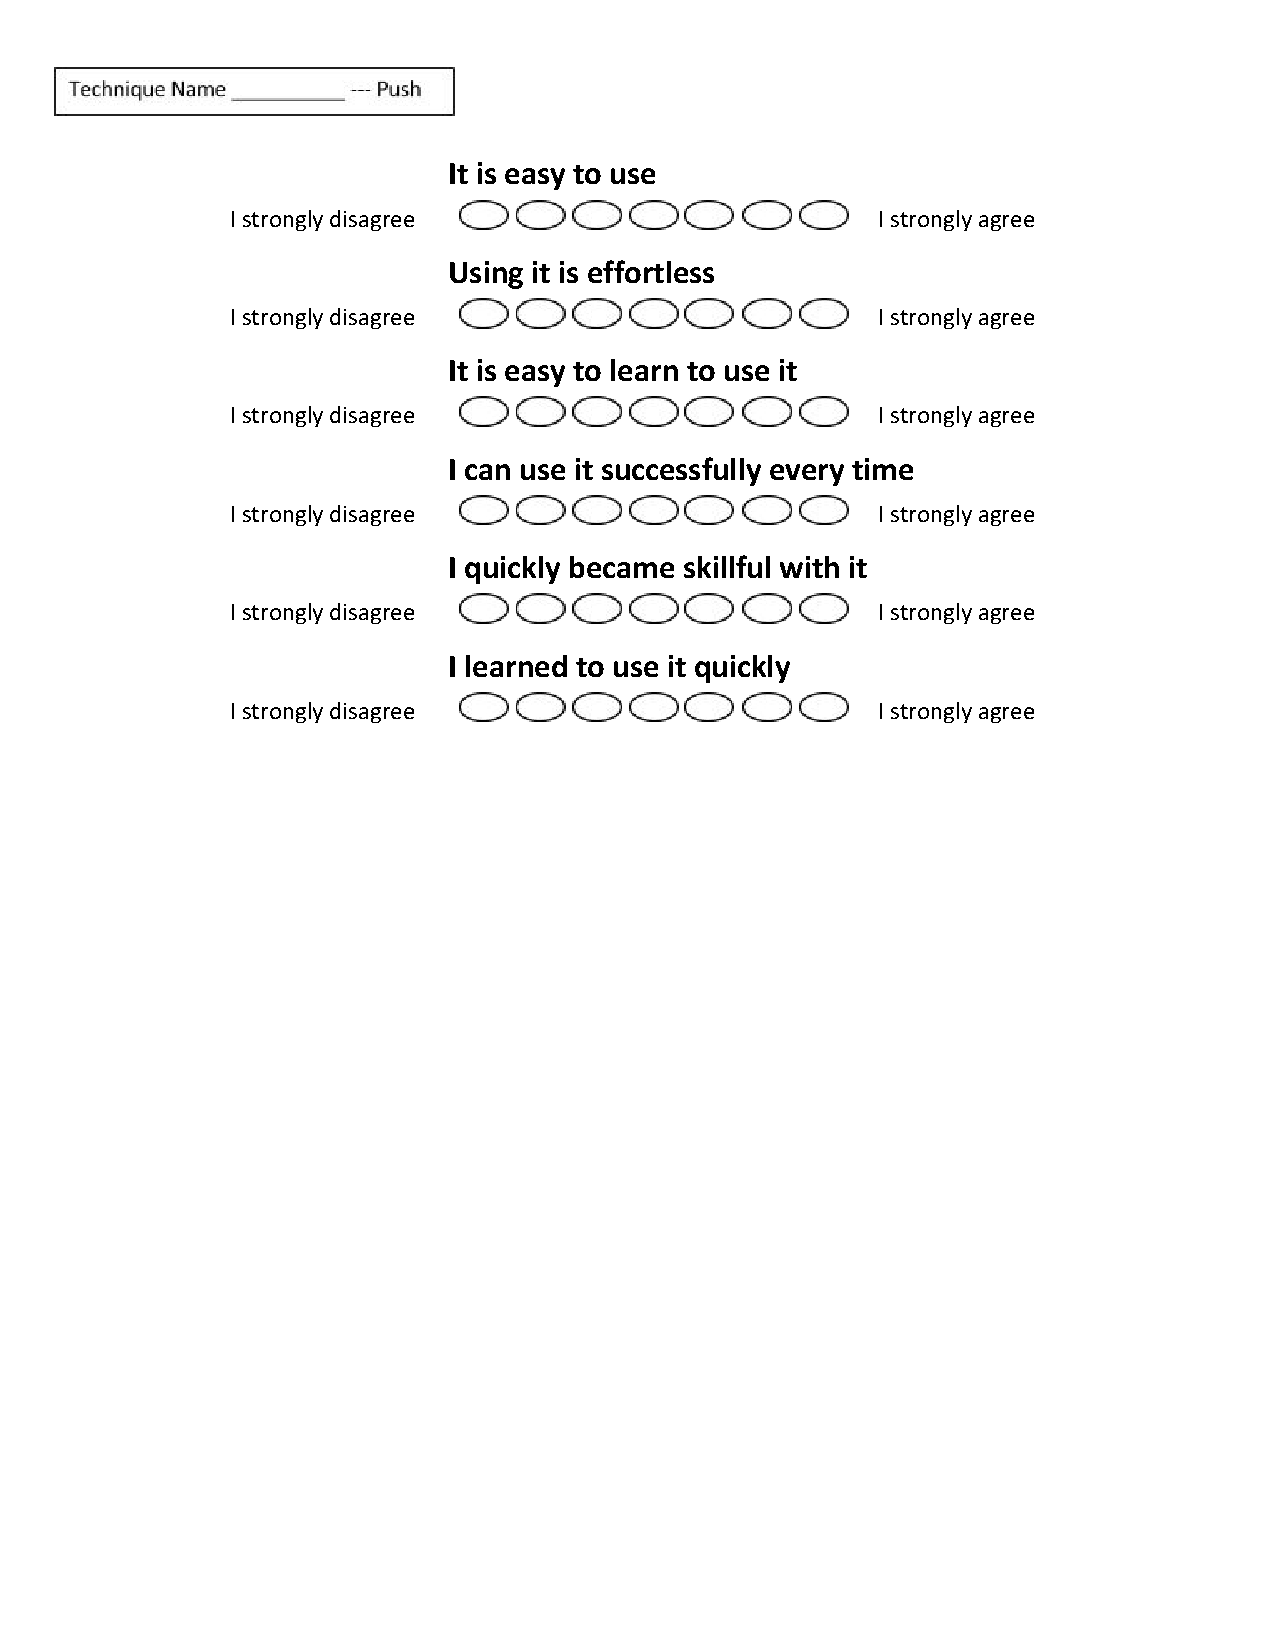
\includepdf[clip,trim=0cm 0cm 0cm -6cm,pages={1},pagecommand={\section*{Appendix A: Questionnaire}}]{images/questionnaire.pdf} 

\newpage\null\thispagestyle{empty}\newpage
\cleardoublepage

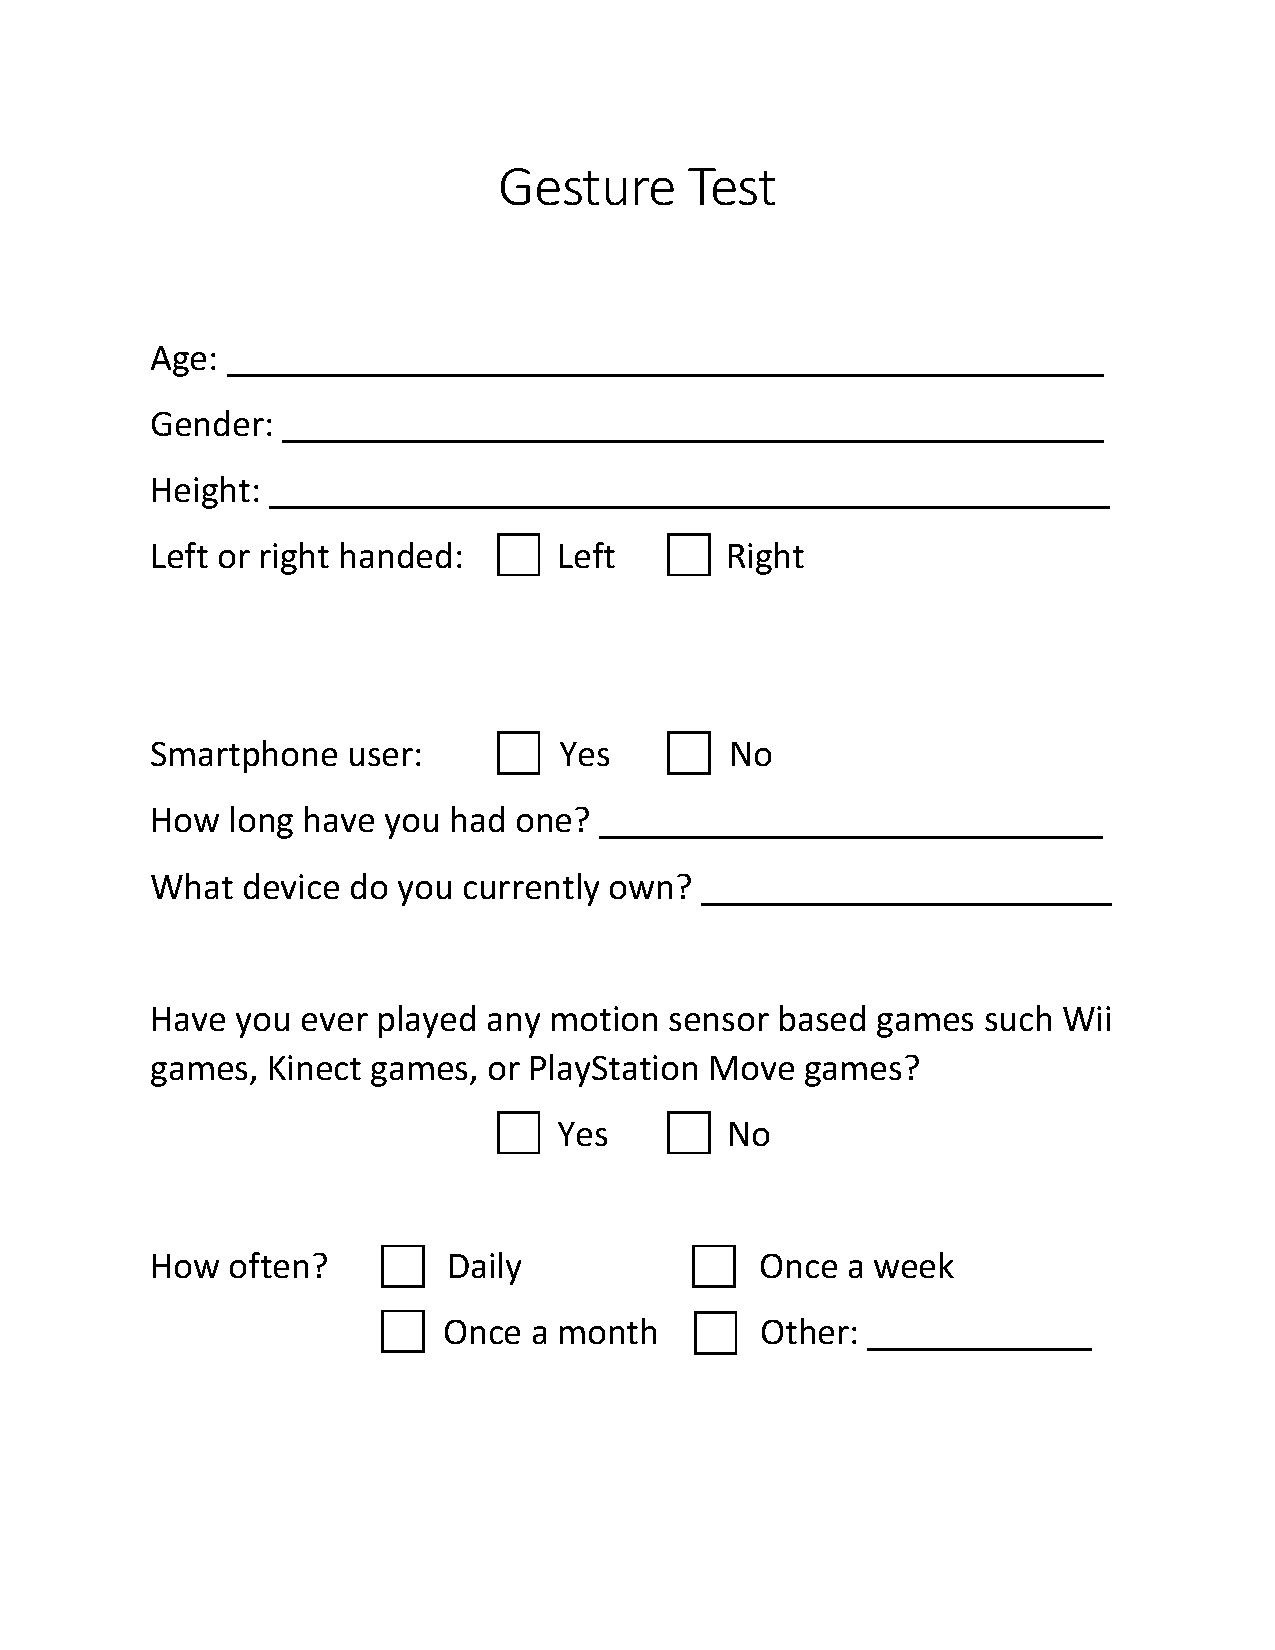
\includepdf[clip,trim=0cm 0cm 0cm -4cm,pages={1},pagecommand={\subsection{Appendix B: Demographic Questionnaire}}]{appendix/images/demographics.pdf} 

\newpage\null\thispagestyle{empty}\newpage
\cleardoublepage

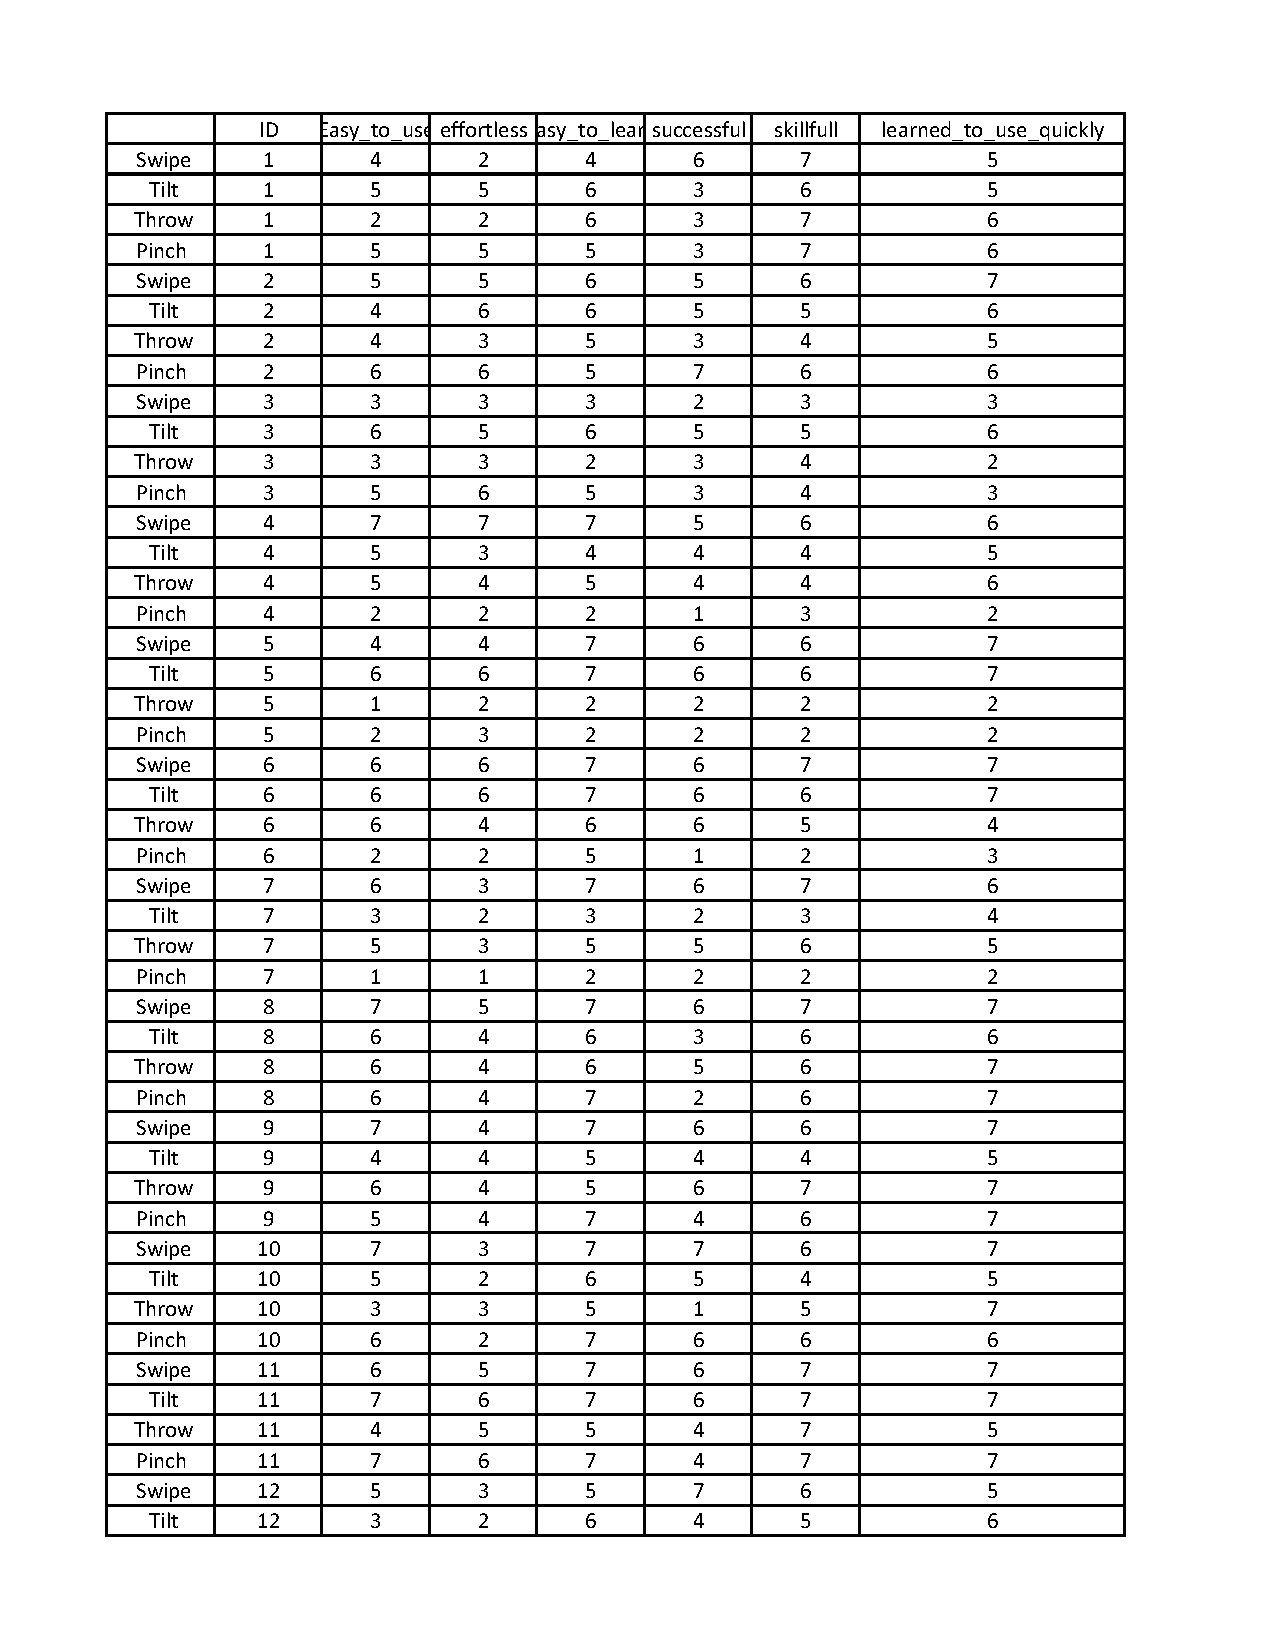
\includepdf[scale=0.95,clip,trim=0cm 0cm 0cm -2cm,pages={1},pagecommand={\subsection*{Appendix C: Questionnaire Results}\addcontentsline{toc}{subsection}{Appendix C: Questionnaire Results}}]{appendix/images/questionnairesurvey.pdf} 
\includepdf[scale=0.95,clip,trim=0cm 0cm 0cm 0cm,pages={2-last},pagecommand={}]{appendix/images/questionnairesurvey.pdf}

\newpage\null\thispagestyle{empty}\newpage
\cleardoublepage

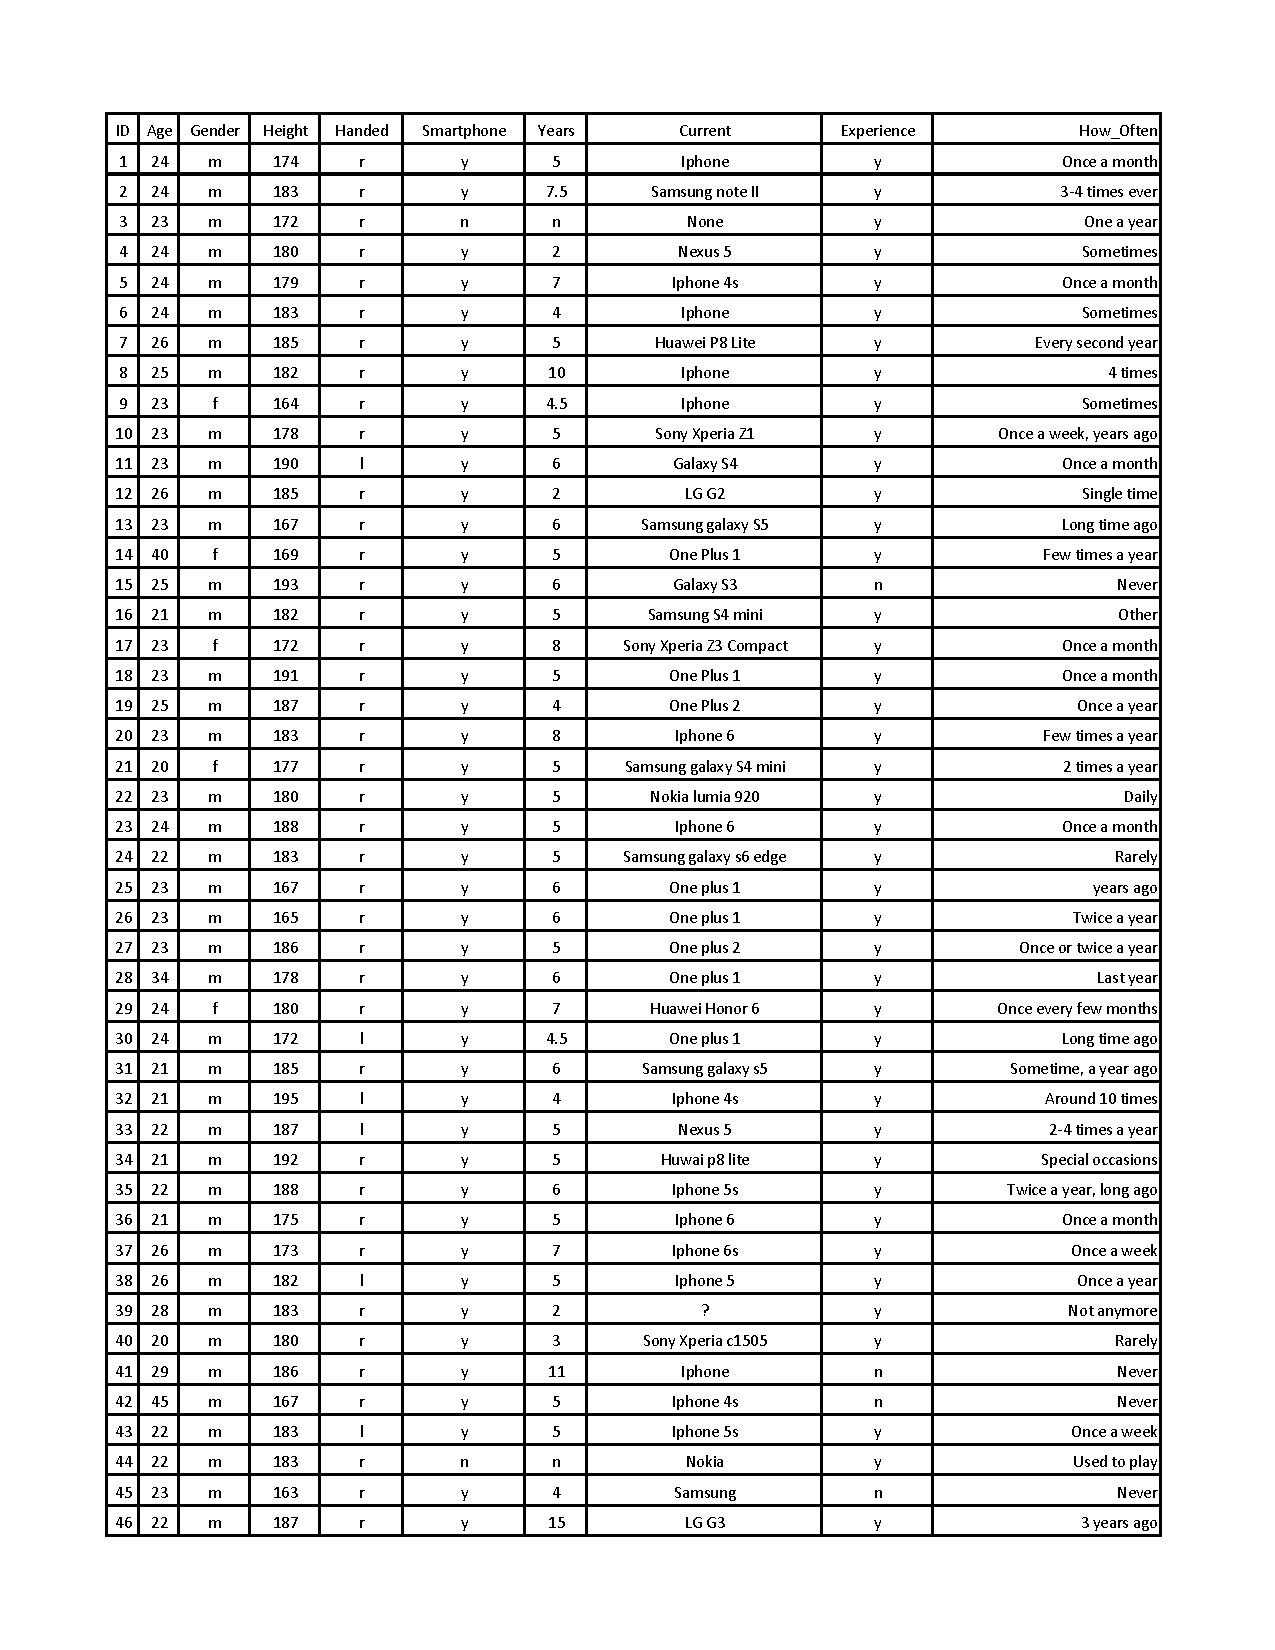
\includepdf[scale=0.95,clip,trim=0cm 0cm 0cm -2cm,pages={1},pagecommand={\subsection{Appendix D: Demographic Results}}]{appendix/images/demosurvey.pdf} 
\includepdf[scale=0.95,clip,trim=0cm 0cm 0cm 0cm,pages={2},pagecommand={}]{appendix/images/demosurvey.pdf}

\subsection{Appendix E: Example of raw comment log}
\verbatiminput{appendix/images/rawcomments.txt}

\newpage\null\thispagestyle{empty}\newpage
\cleardoublepage

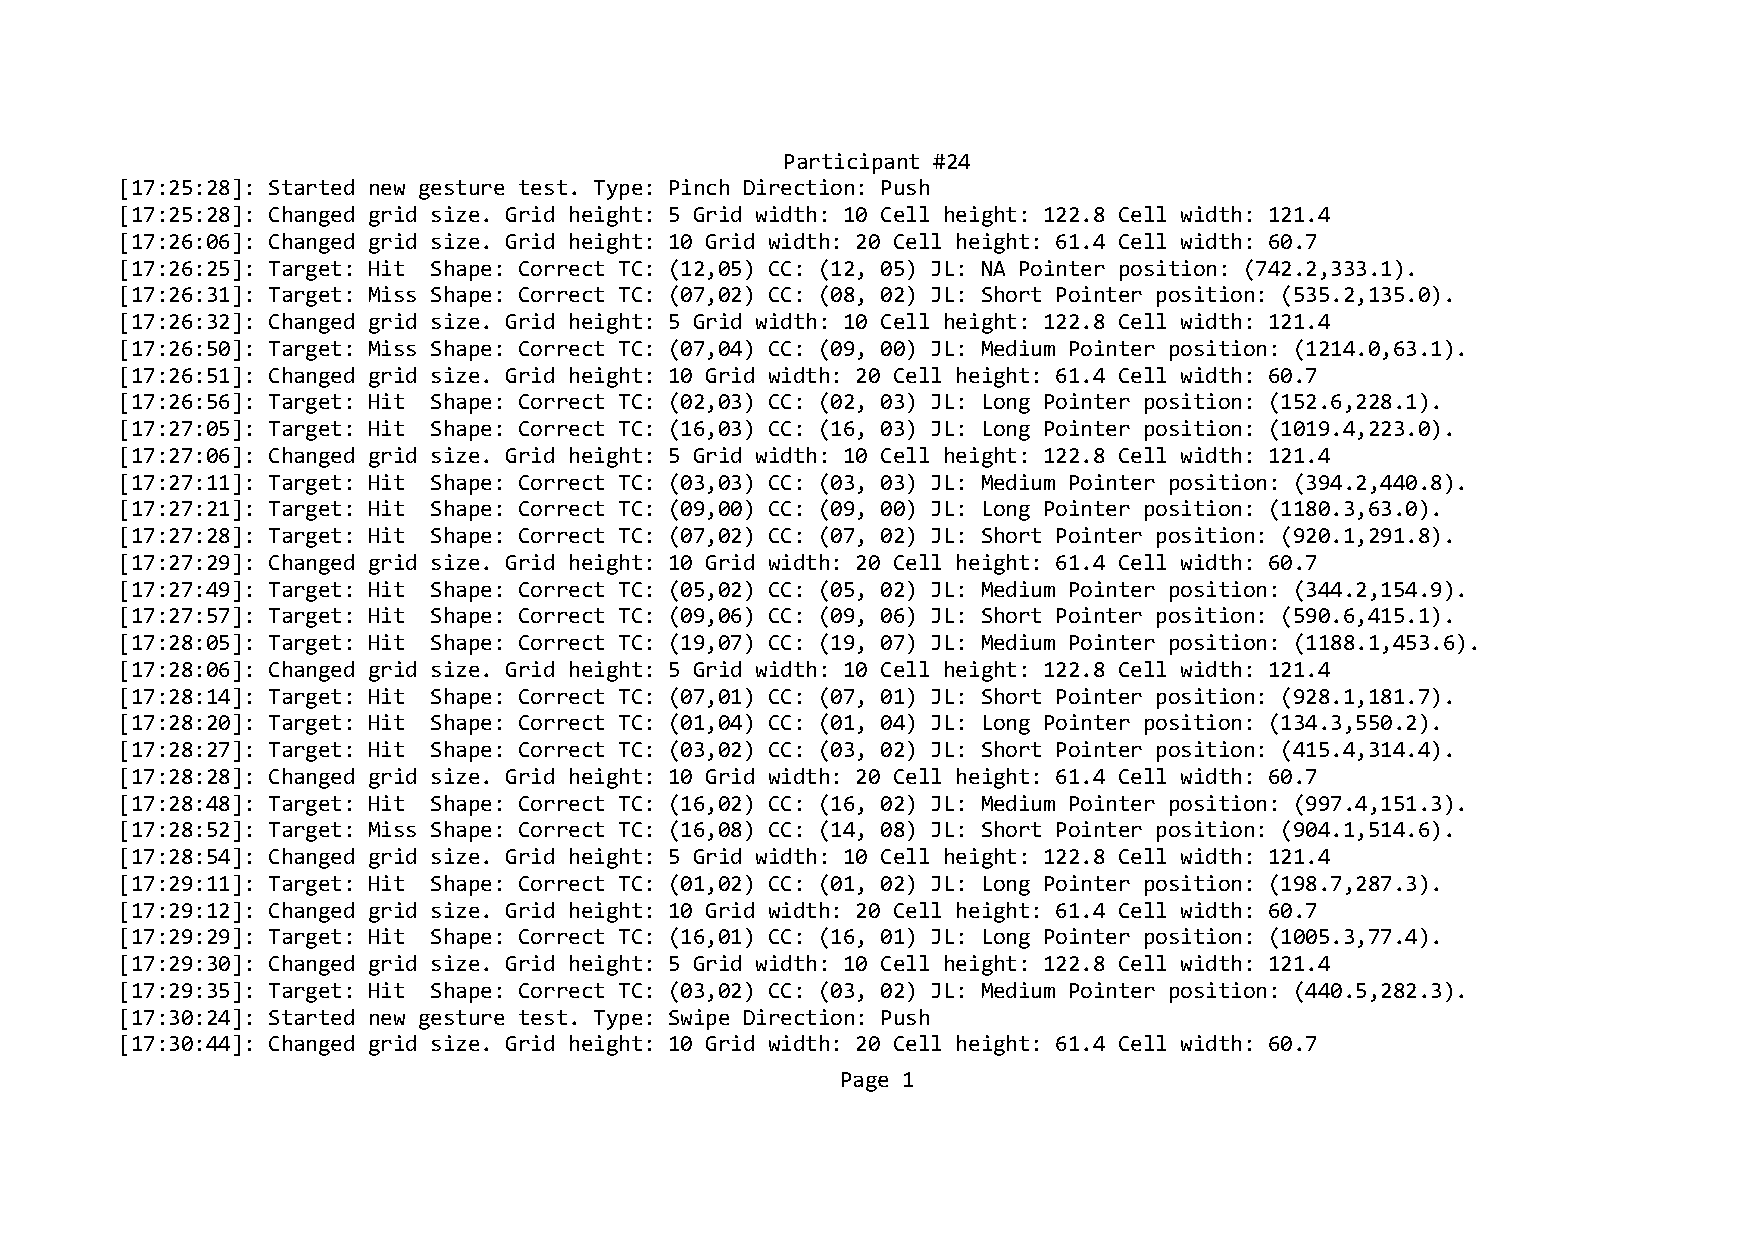
\includepdf[landscape=true,clip,trim=0cm 0cm 0cm -4cm,pages={1},pagecommand={\section*{Appendix F: Example of raw test log}}]{images/log.pdf} 
\includepdf[landscape=true,clip,trim=0cm 0cm 0cm -4cm,pages={2-last},pagecommand={}]{images/log.pdf}

\section{Appendix G: Recruitment Poster}
\begin{adjustbox}{width=\textwidth}
	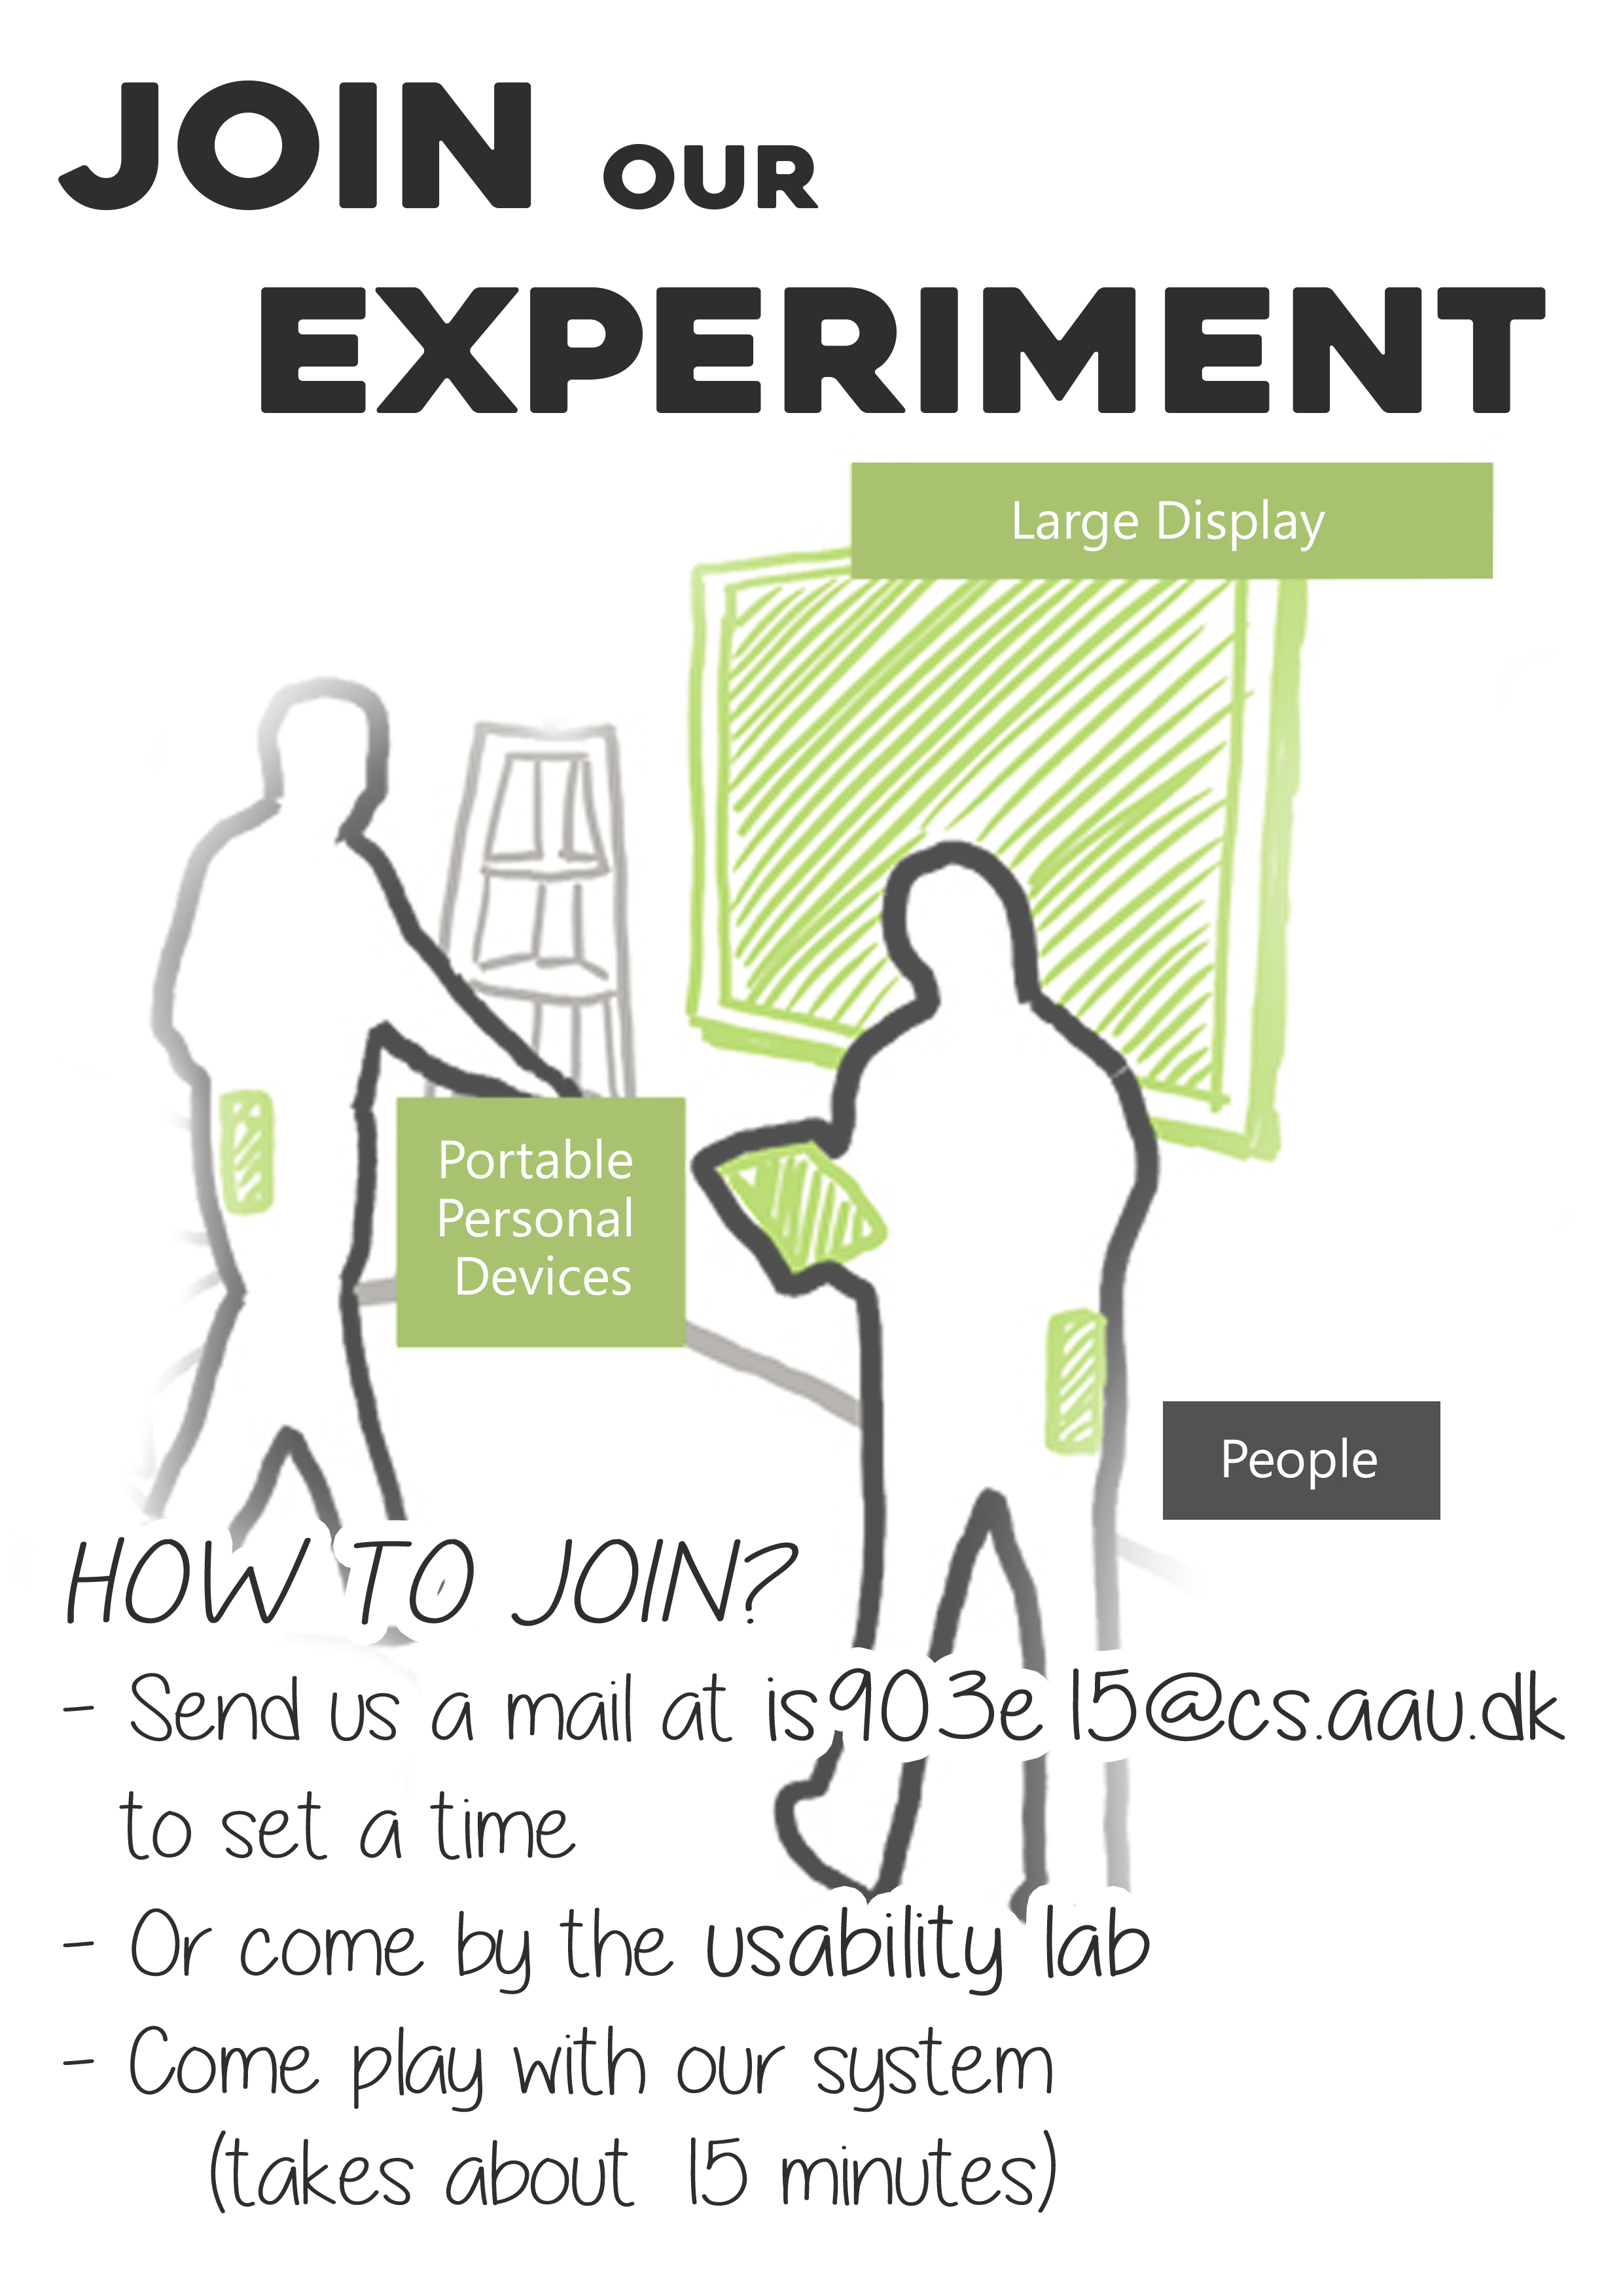
\includegraphics{images/poster.jpg}
\end{adjustbox}

\thispagestyle{empty}
\cleardoublepage

\subsection*{Appendix H: Pictures}
\addcontentsline{toc}{subsection}{Appendix H: Pictures}

\subsection*{Setup}
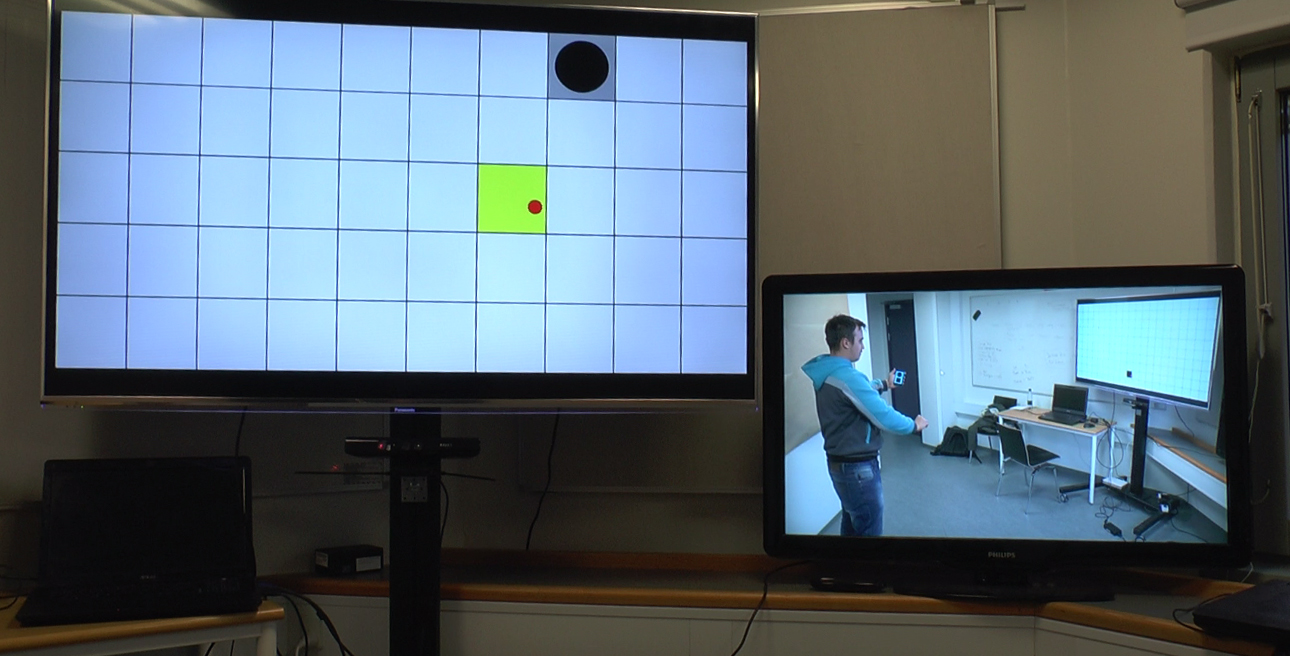
\includegraphics[width=\textwidth]{appendix/images/setup.jpg}

\subsection*{Presenting the experiment}
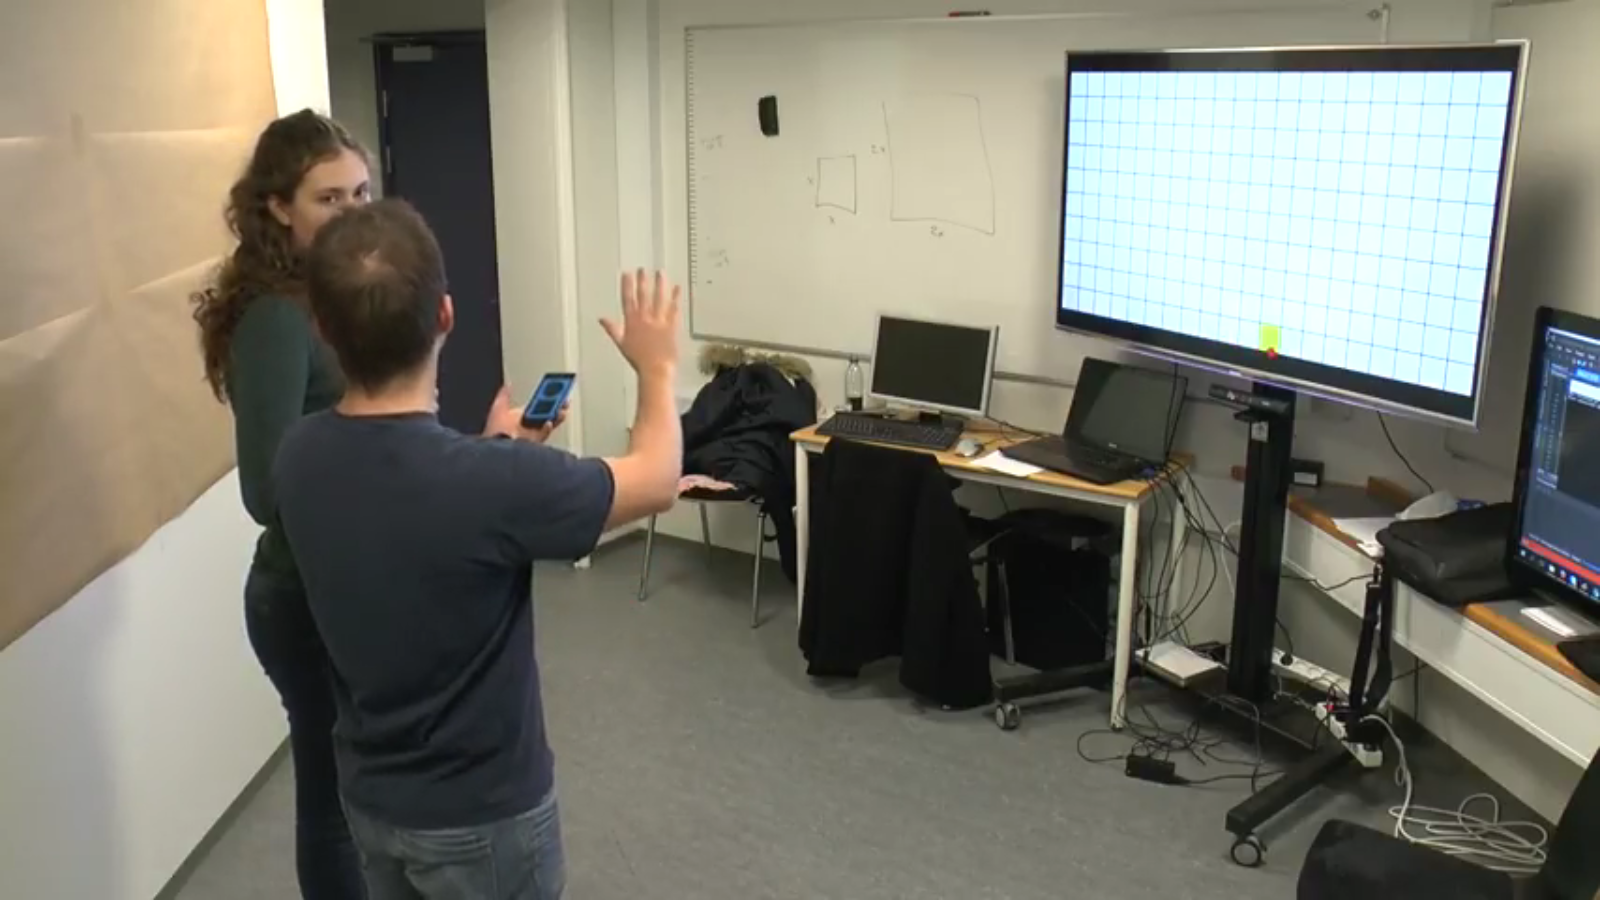
\includegraphics[width=\textwidth]{appendix/images/alina_presenting.png}

\subsection*{Pinch technique}
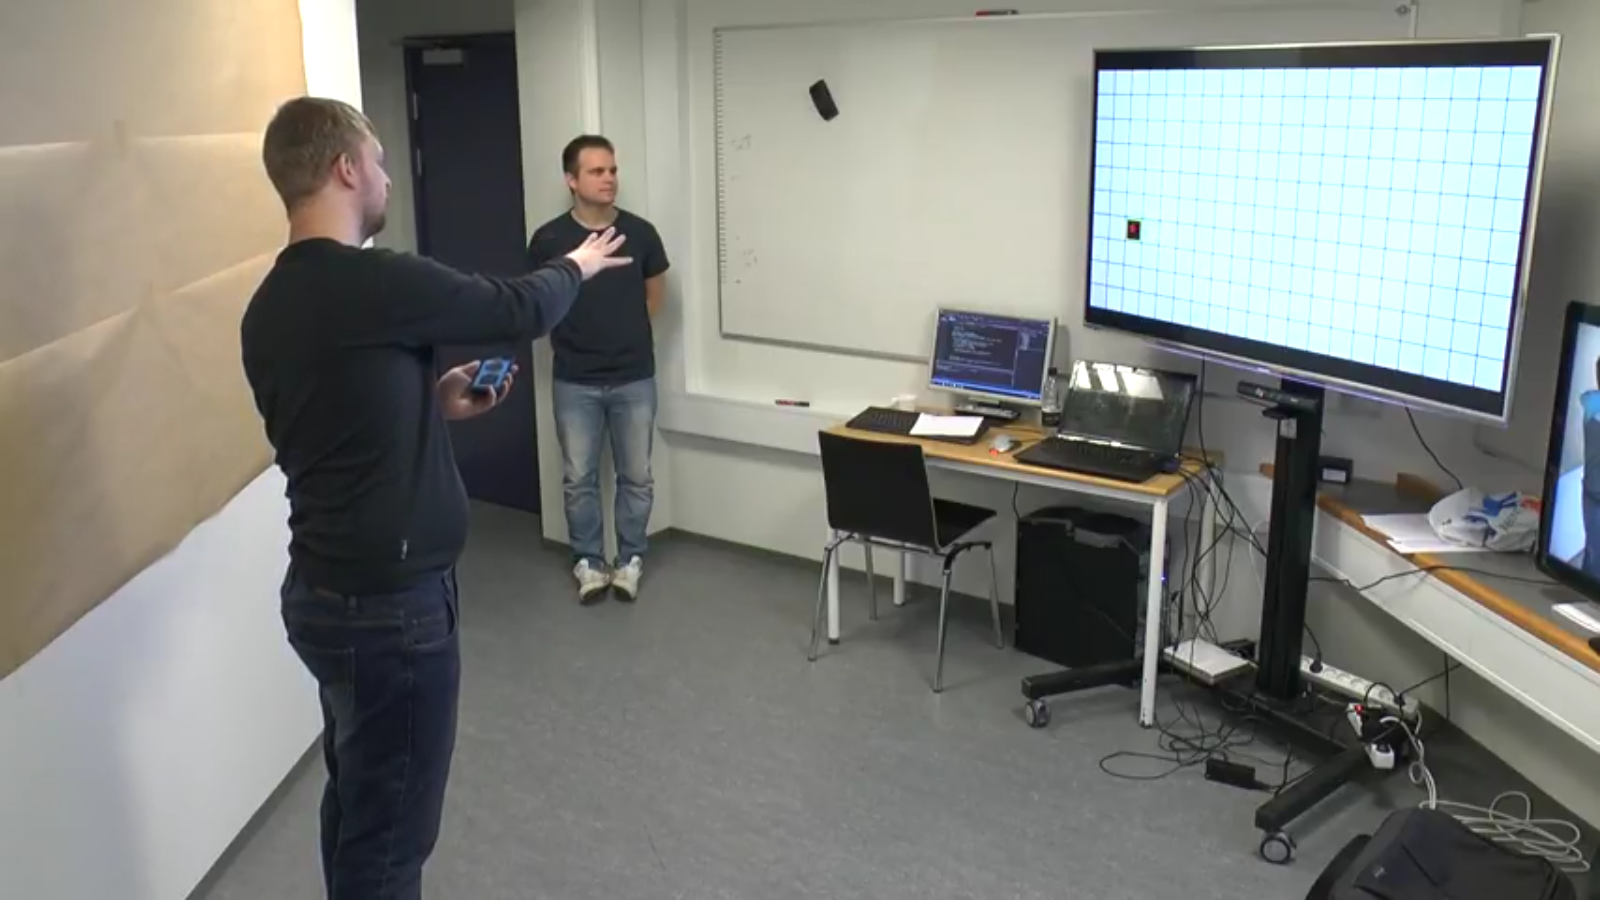
\includegraphics[width=\textwidth]{appendix/images/alex_pinching.png}

\subsection*{Pinch technique}
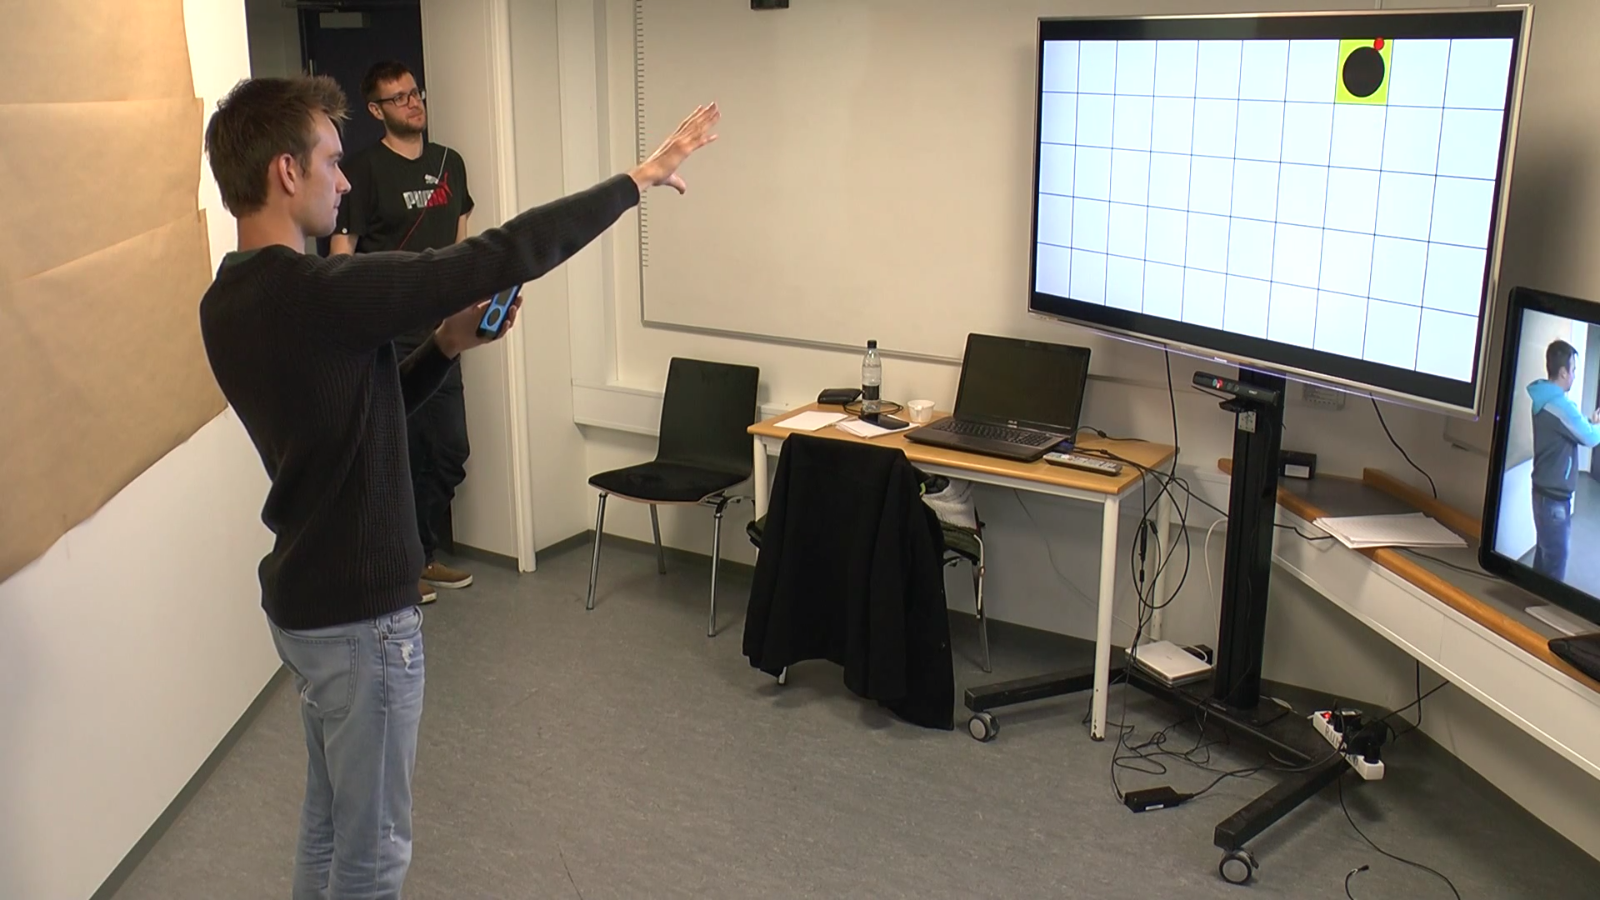
\includegraphics[width=\textwidth]{appendix/images/steffen_pinch.png}

\subsection*{Swipe technique}
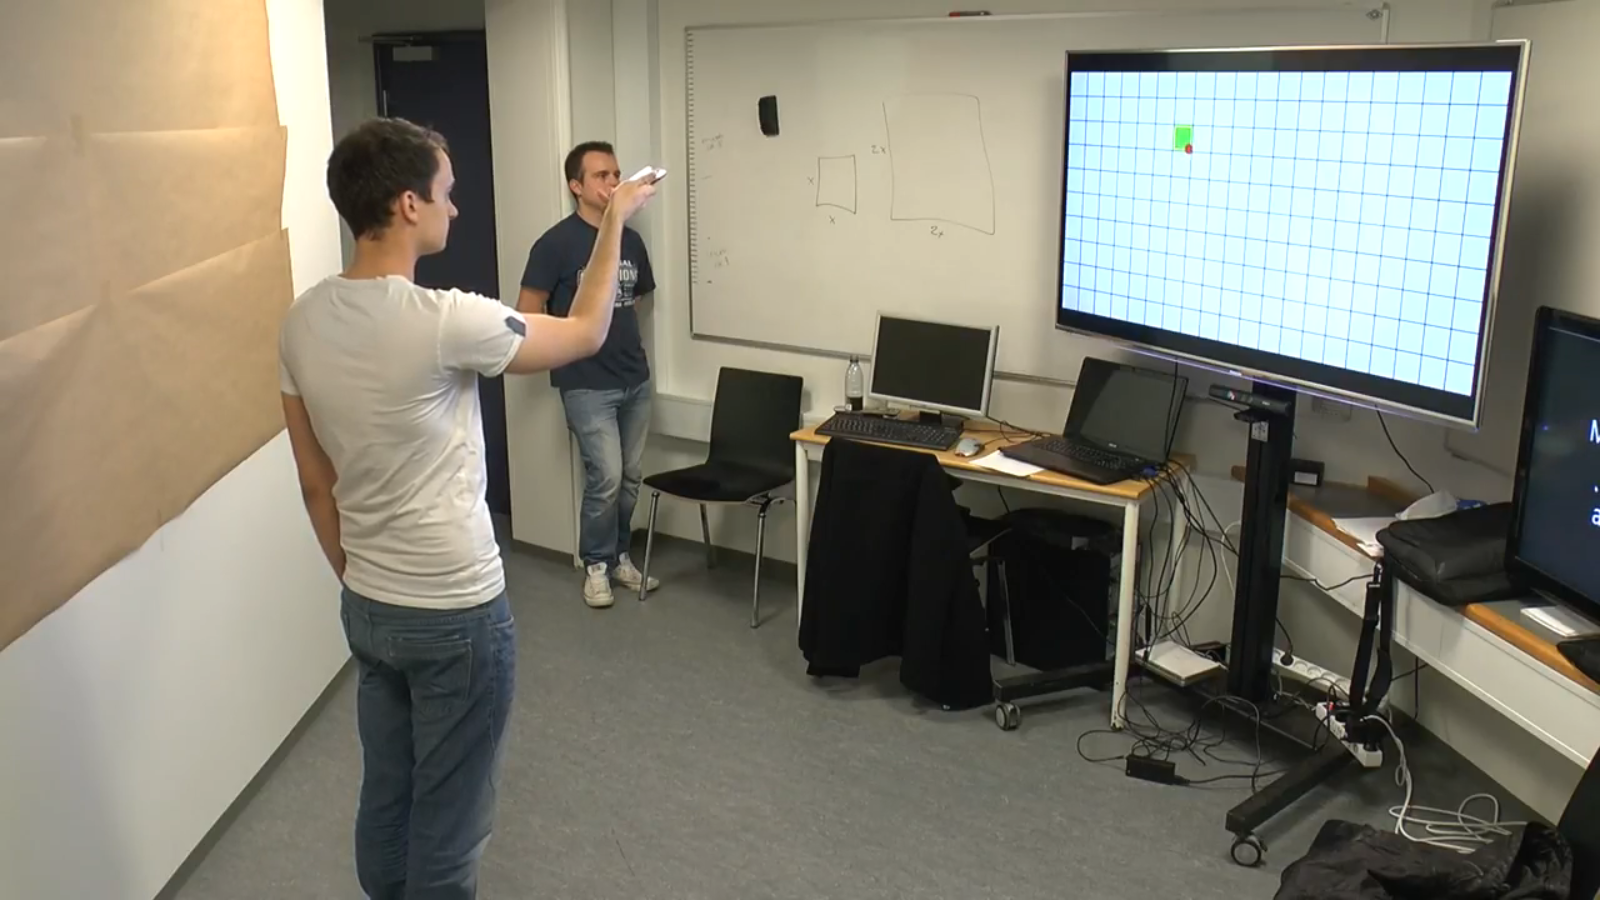
\includegraphics[width=\textwidth]{appendix/images/mathias_swipe.png}

\subsection*{Throw technique}
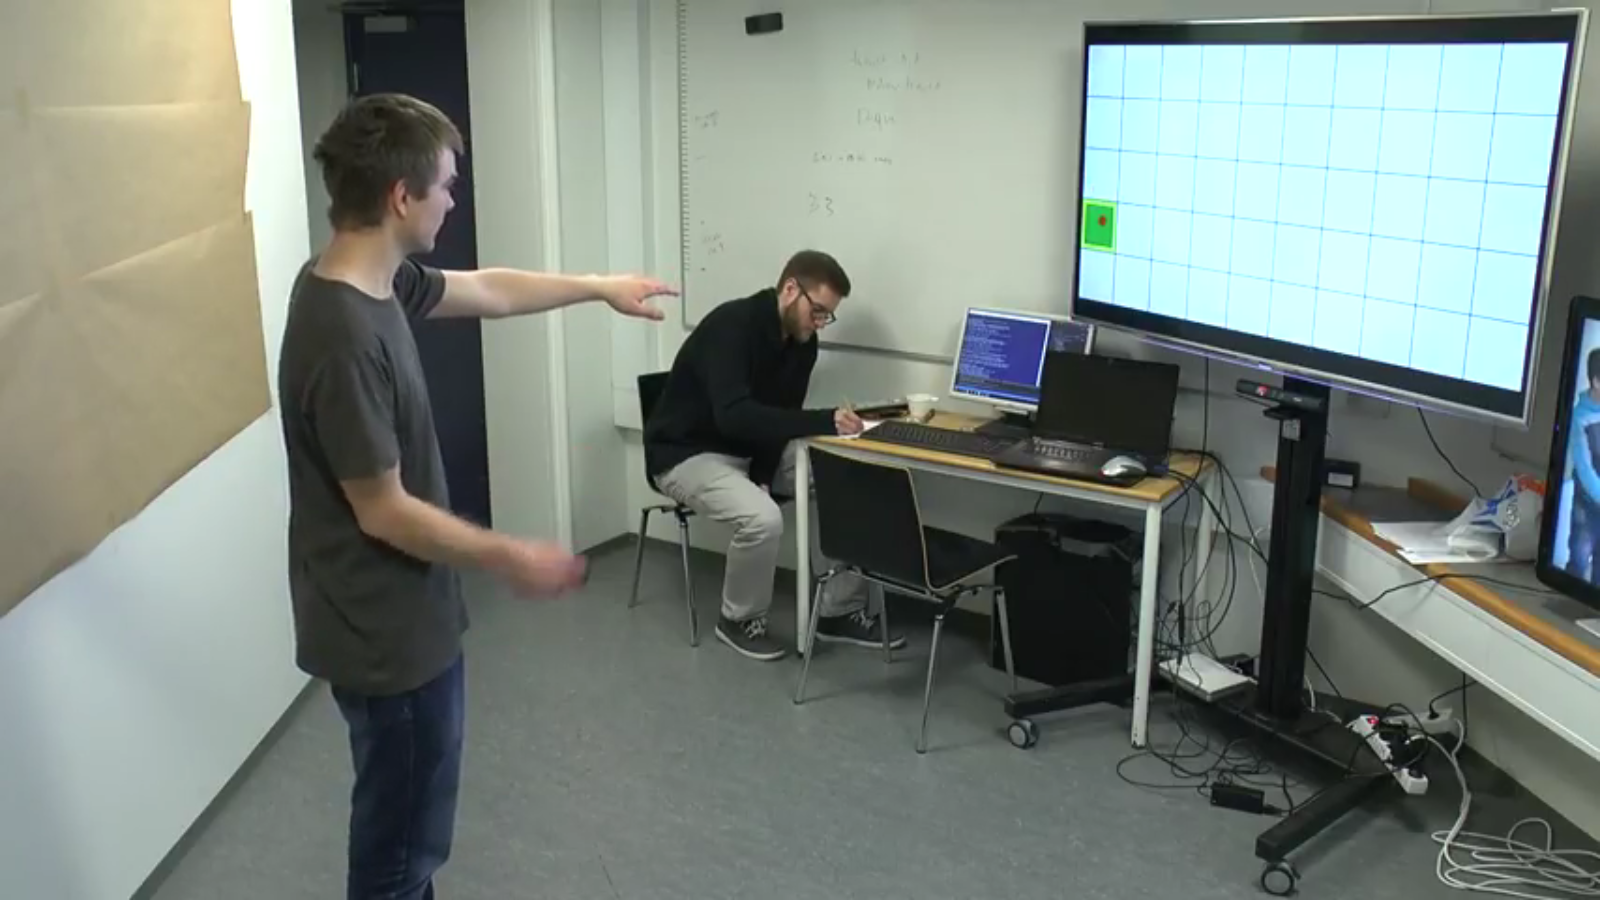
\includegraphics[width=\textwidth]{appendix/images/christian_throwing.png}

\subsection*{Throw technique}
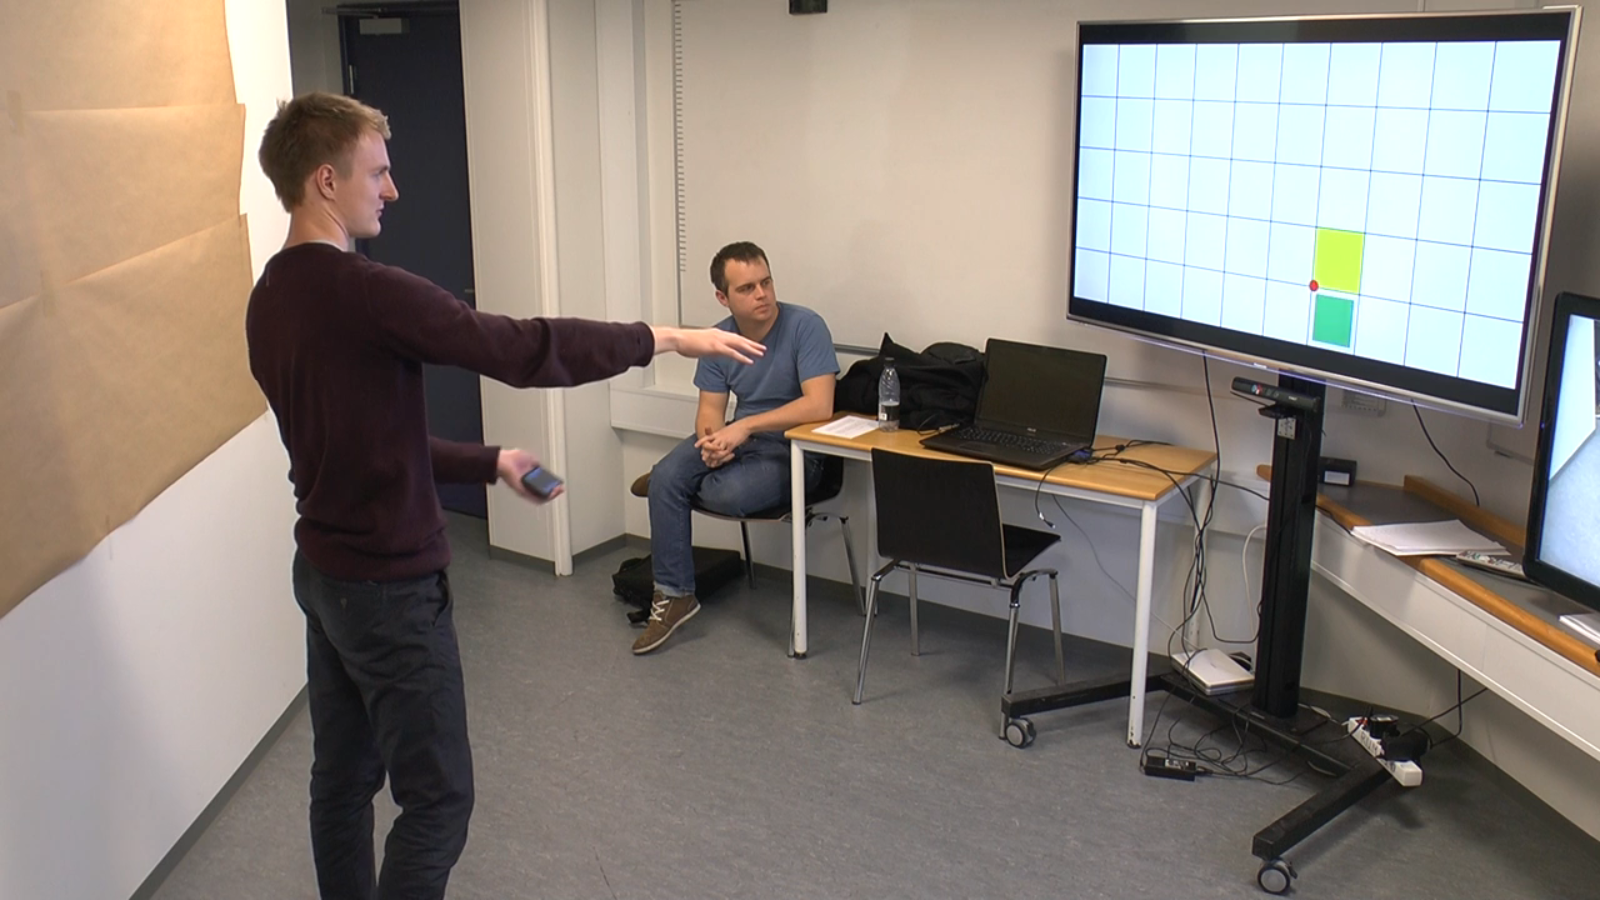
\includegraphics[width=\textwidth]{appendix/images/sune_nilausen_throw.png}

\subsection*{Tilt technique}
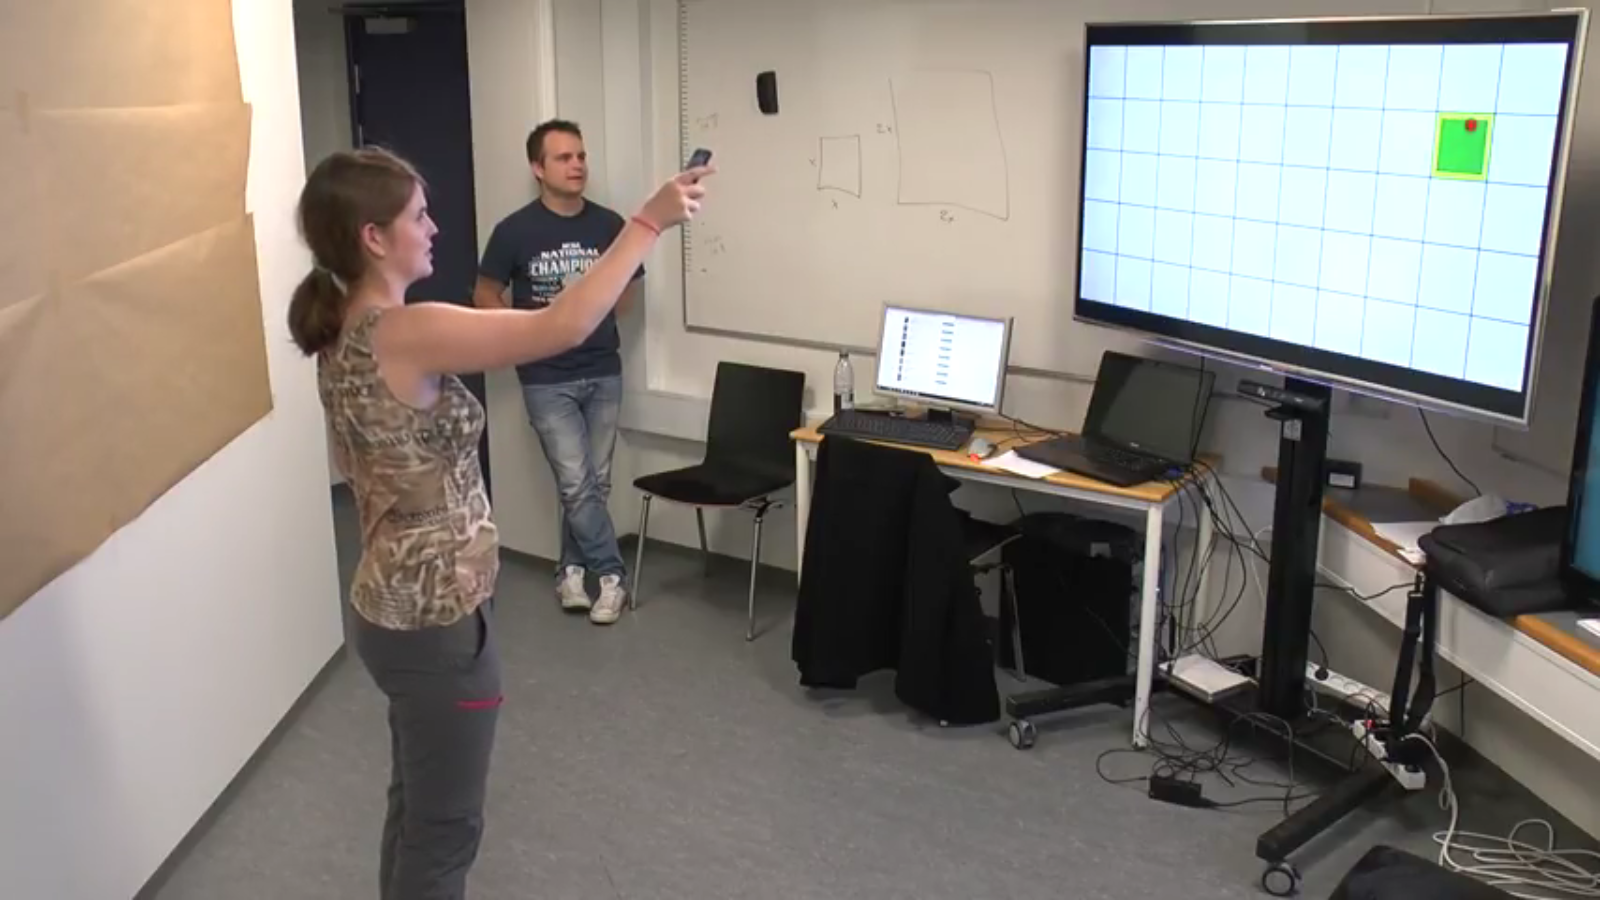
\includegraphics[width=\textwidth]{appendix/images/mette_tilt.png}

\subsection*{Participant on a chair}
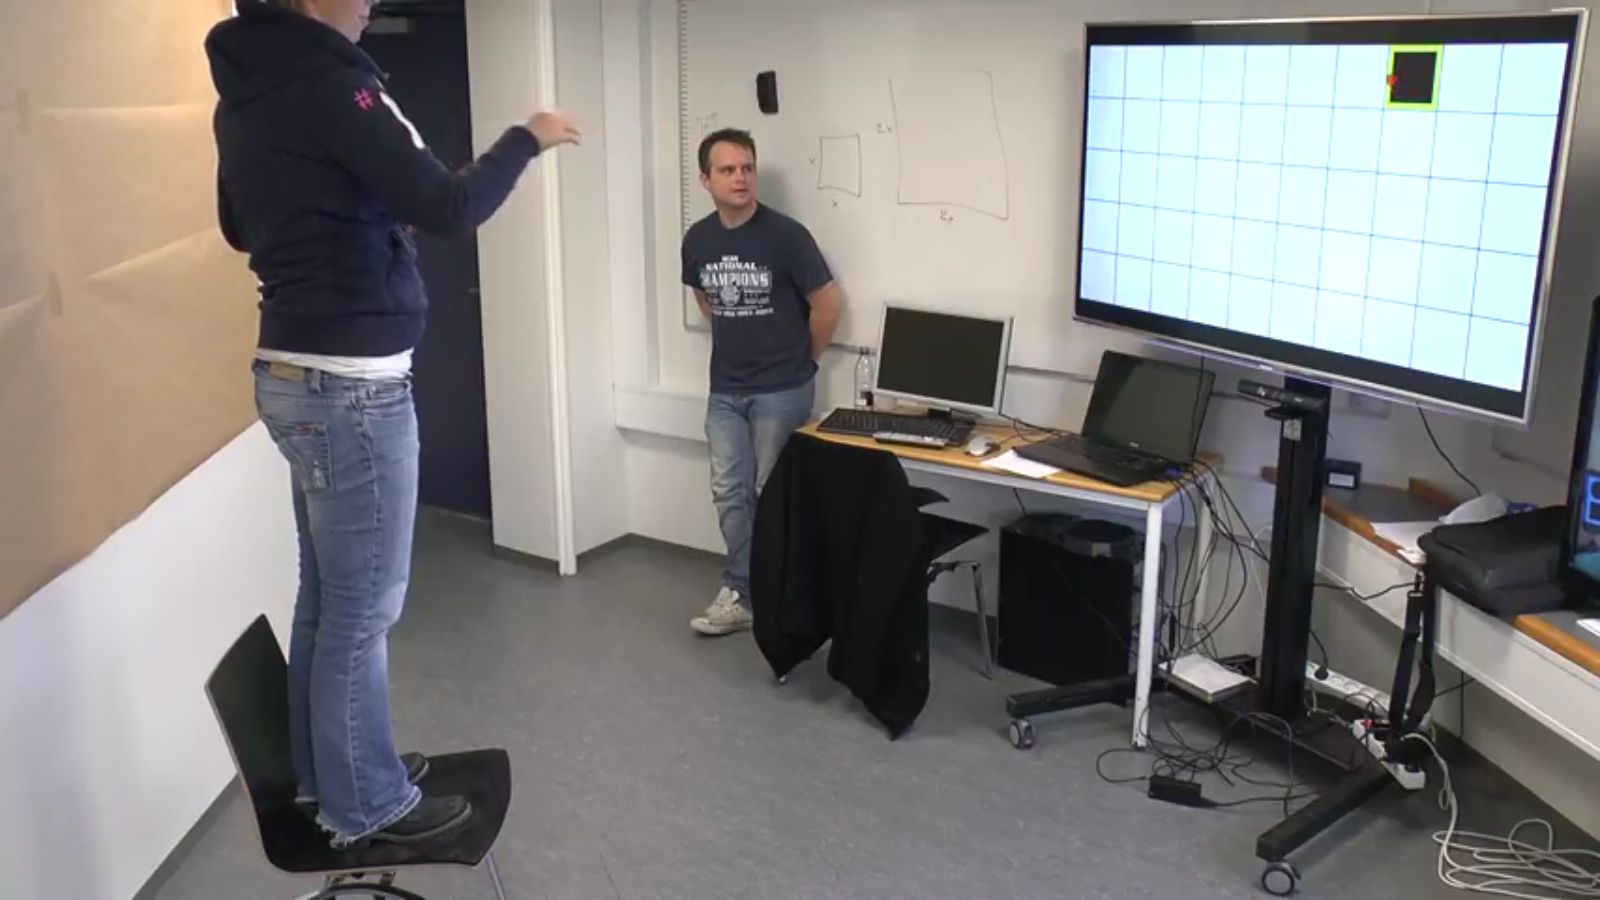
\includegraphics[width=\textwidth]{appendix/images/rikke_on_chair.png}

\subsection*{Pilot test}
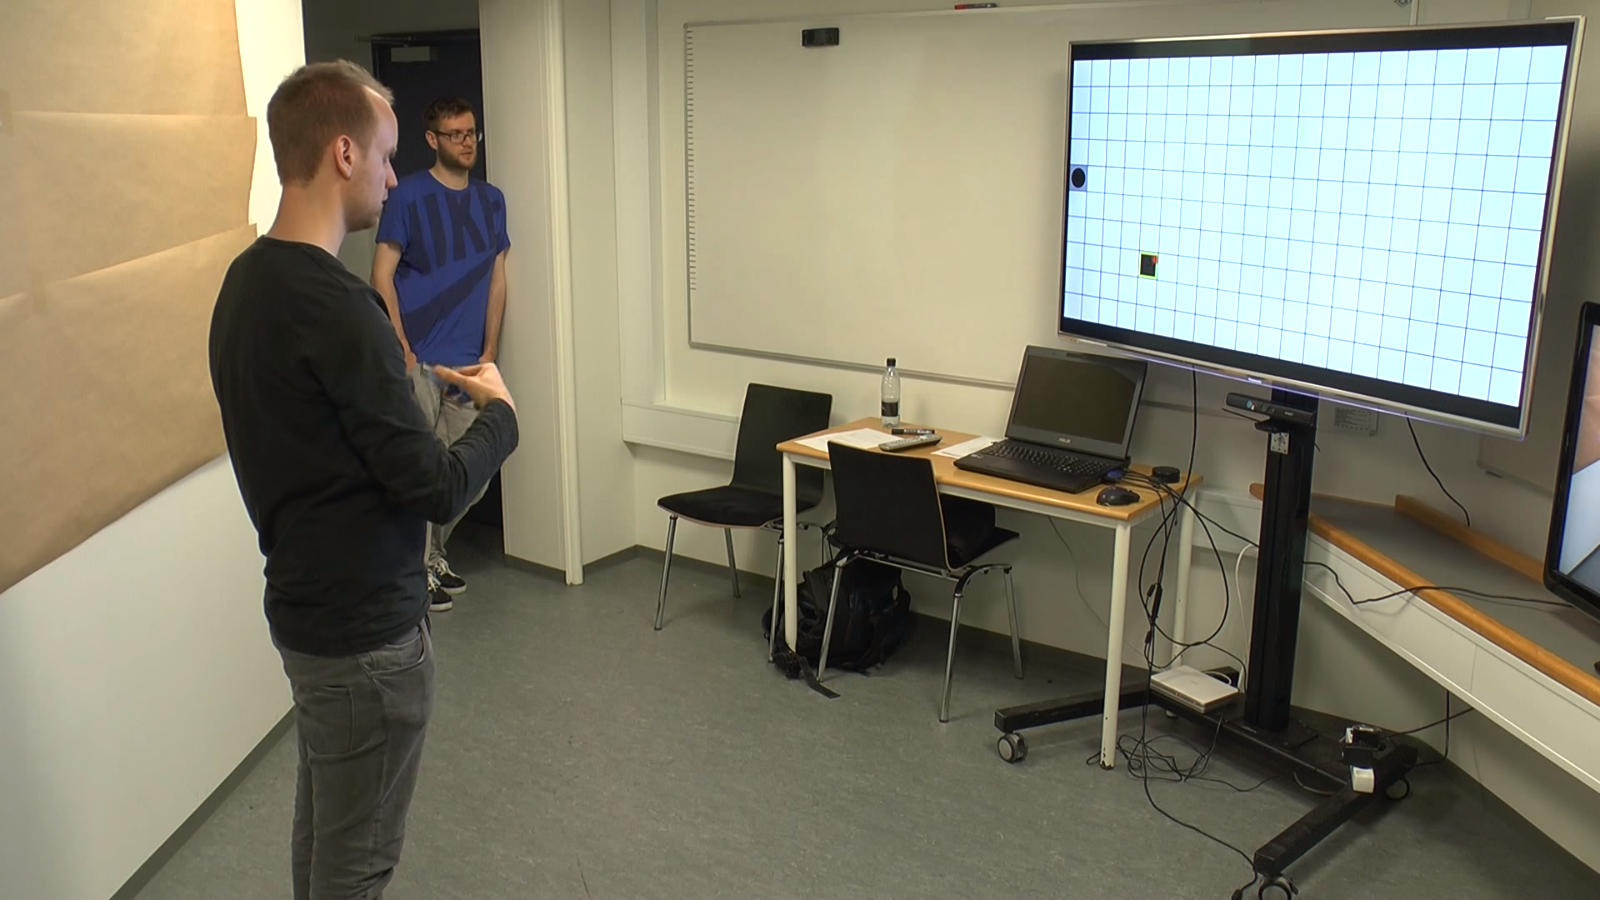
\includegraphics[width=\textwidth]{appendix/images/rune_pilot.png}
%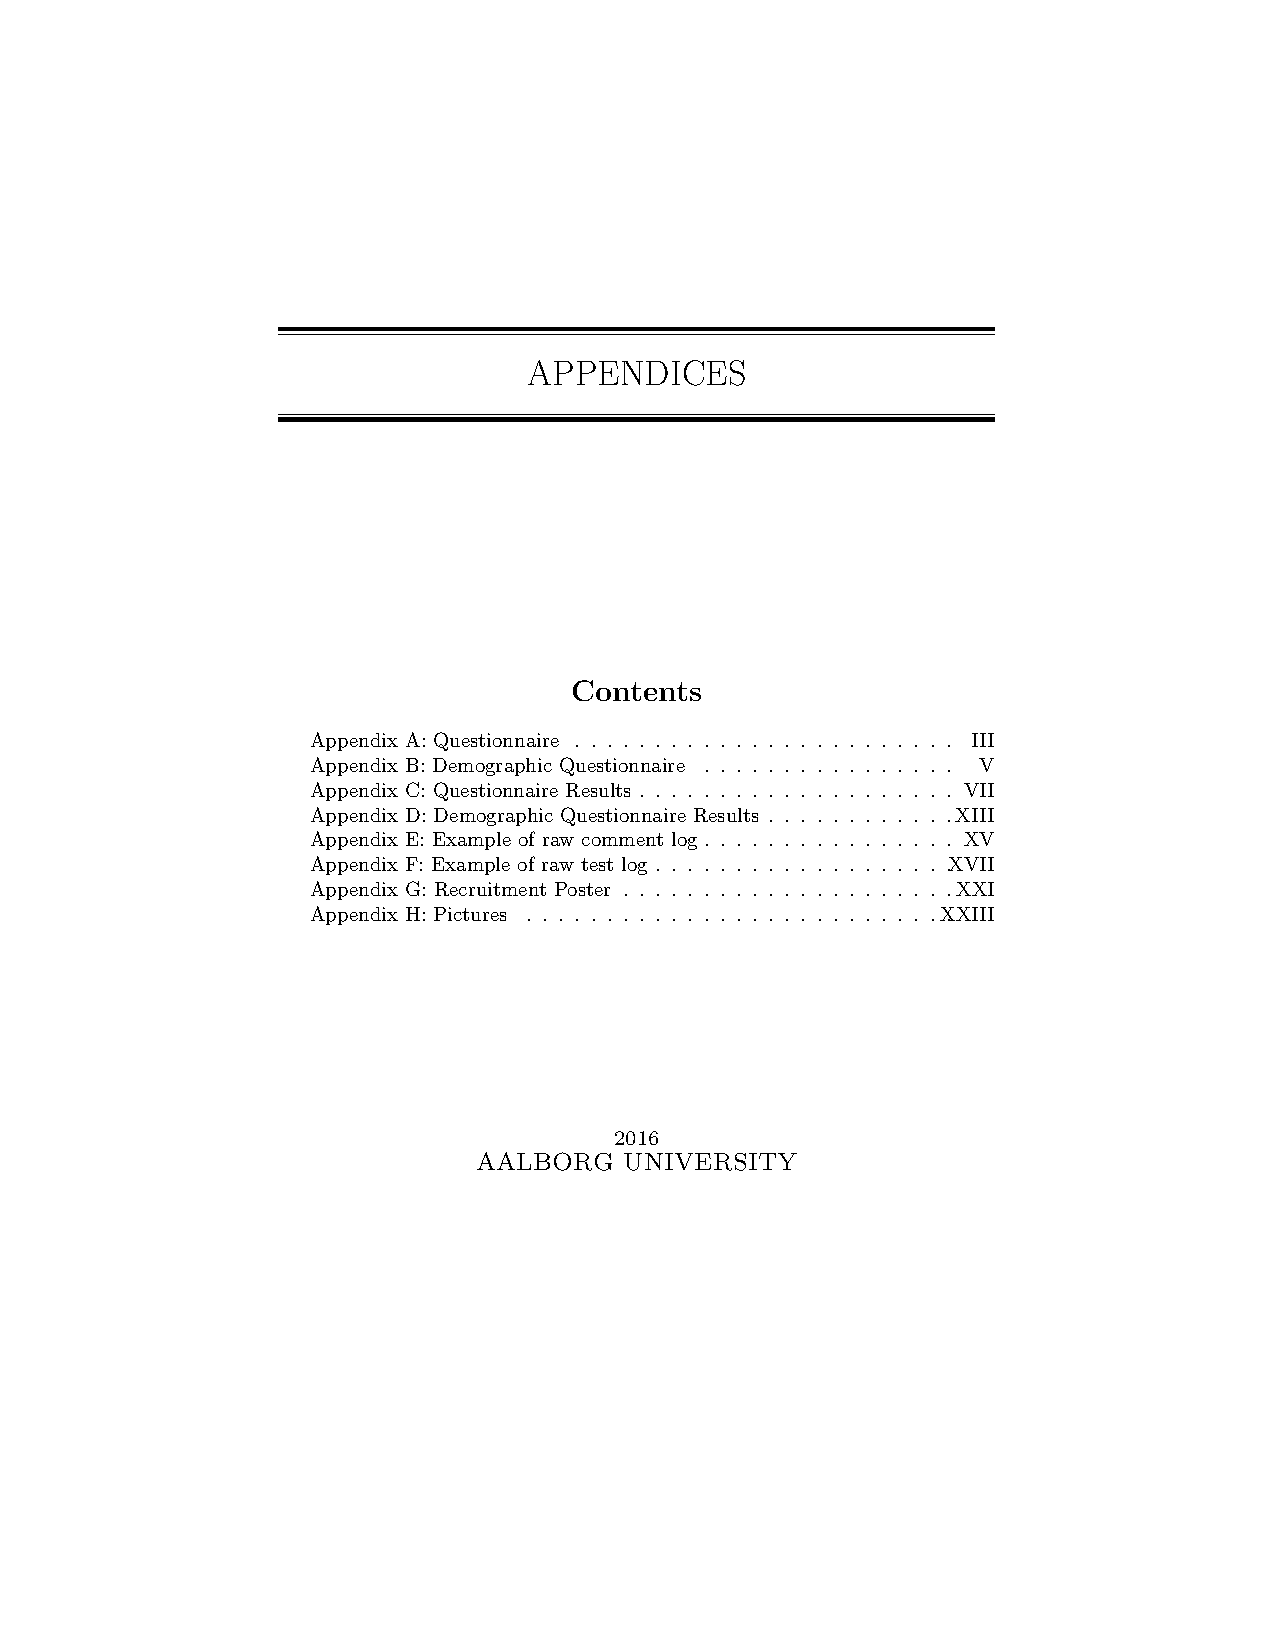
\includepdf[pages=-,pagecommand={\thispagestyle{customplain}},fitpaper,rotateoversize]{appendix/appendix.pdf}
%OR
%\includepdf[pages=1-,pagecommand={\thispagestyle{fancy}}]{paper1.pdf}
%\includepdf[pages=1-,pagecommand={\thispagestyle{fancy}}]{paper2.pdf}
\end{document}